\documentclass{article} 

% if you need to pass options to natbib, use, e.g.:
% \PassOptionsToPackage{numbers, compress}{natbib}
% before loading nips_2016
%
% to avoid loading the natbib package, add option nonatbib:
% \usepackage[nonatbib]{nips_2016}


\usepackage{dsfont}

% to compile a camera-ready version, add the [final] option, e.g.:
%\usepackage{iclr2018_conference,times}
\usepackage[final]{nips_2017}

\usepackage[utf8]{inputenc} % allow utf-8 input
\usepackage[T1]{fontenc}    % use 8-bit T1 fonts
\usepackage{hyperref}       % hyperlinks
\usepackage{url}            % simple URL typesetting
\usepackage{booktabs}       % professional-quality tables
\usepackage{amsfonts}       % blackboard math symbols
\usepackage{nicefrac}       % compact symbols for 1/2, etc.
\usepackage{microtype}      % microtypography

\usepackage{listings}
\usepackage{amsthm}
% use Times
\usepackage{times}
% For figures
\usepackage{graphicx} % more modern
%\usepackage{epsfig} % less modern
\usepackage{subfig} 
\usepackage{fancyvrb}


\usepackage{caption}
\usepackage{subcaption}

\fvset{fontsize=\footnotesize}

\usepackage{amssymb}
\usepackage{listings}
\usepackage{wrapfig}
\usepackage{tabularx}


\usepackage{verbatim}
 \usepackage{booktabs}
 % For algorithms
\usepackage{algorithm}
\usepackage{algorithmic}
\usepackage{tikz}
\usetikzlibrary{fit}
\usetikzlibrary{arrows.meta}
\usetikzlibrary{positioning}
\usetikzlibrary{decorations.text,decorations.pathreplacing}
\usetikzlibrary{decorations.pathmorphing}

% As of 2011, we use the hyperref package to produce hyperlinks in the
% resulting PDF.  If this breaks your system, please commend out the
% following usepackage line and replace \usepackage{icml2016} with
% \usepackage[nohyperref]{icml2016} above.
\usepackage{amsmath}
\usepackage{hyperref}
\DeclareMathOperator*{\argmin}{arg\,min} % thin space, limits underneath in displays
\DeclareMathOperator*{\argmax}{arg\,max} % thin space, limits underneath in displays
\DeclareMathOperator{\argmin}{argmin} % no space, limits underneath in displays



% Packages hyperref and algorithmic misbehave sometimes.  We can fix
% this with the following command.

\newcommand{\Expect}{\mathds{E}} %{{\rm I\kern-.3em E}}
\newcommand{\indicator}{\mathds{1}} %{{\rm I\kern-.3em E}}
\newcommand{\expect}{\mathds{E}} %{{\rm I\kern-.3em E}}
\newcommand{\probability}{\mathds{P}} %{{\rm I\kern-.3em P}}

\newtheorem{proposition}{Proposition}

\newcommand\modt{\stackrel{\mathclap{\normalfont 2}}{\equiv}}


\title{Supplement to: Learning to Infer Graphics Programs from Hand-Drawn Images}

% The \author macro works with any number of authors. There are two
% commands used to separate the names and addresses of multiple
% authors: \And and \AND.
%
% Using \And between authors leaves it to LaTeX to determine where to
% break the lines. Using \AND forces a line break at that point. So,
% if LaTeX puts 3 of 4 authors names on the first line, and the last
% on the second line, try using \AND instead of \And before the third
% author name.

\author{
Kevin Ellis\\
  MIT\\
  \texttt{ellisk@mit.edu} \\
  \And
  Daniel Ritchie\\
Brown University\\
 \texttt{daniel\_ritchie@brown.edu} \\
 \And
 Armando Solar-Lezama\\
 MIT\\
\texttt{asolar@csail.mit.edu} \\
\And
Joshua B. Tenenbaum \\
MIT\\
\texttt{jbt@mit.edu}
  %% Affiliation \\
  %% Address \\
  %% \texttt{email} \\
  %% \And
  %% Coauthor \\
  %% Affiliation \\
  %% Address \\
  %% \texttt{email} \\
  %% \And
  %% Coauthor \\
  %% Affiliation \\
  %% Address \\
  %% \texttt{email} \\
}

\begin{document}
% \nipsfinalcopy is no longer used

\maketitle

\section{Neural network architecture and training}

\subsection{High-level overview}

For the model in Fig.~\ref{architecture}, the distribution over the next drawing command factorizes as:
\begin{equation}
  \probability_\theta [t_1t_2\cdots t_K | I,S] = \prod_{k = 1}^K \probability_\theta \left[t_k | a_\theta \left(f_\theta(I,\text{render}(S)) | \{t_j\}_{j = 1}^{k - 1}\right), \{t_j\}_{j = 1}^{k - 1}\right]
\end{equation}
where $t_1t_2\cdots t_K$ are the tokens in the drawing command, $I$ is
the target image, $S$ is a spec, $\theta$ are the
parameters of the neural network, $f_\theta(\cdot,\cdot)$ is the
image feature extractor (convolutional network), and $a_\theta(\cdot|\cdot)$ is an attention mechanism. The distribution over
specs factorizes as:
\begin{equation}
  \probability_\theta [S|I] = \prod_{n = 1}^{|S|} \probability_\theta [S_n | I,S_{1:(n-1)}]\times\probability_\theta [\verb|STOP| | I,S]\label{objective}
\end{equation}
where $|S|$ is the length of spec $S$, the subscripts
on $S$ index drawing commands within the spec (so $S_n$ is a sequence of tokens: $t_1t_2\cdots t_K$), and the \verb|STOP|
token is emitted by the network to signal that the spec
explains the image.
\tikzset{>=latex}
\begin{figure}
  \begin{tikzpicture}
  \node[draw,blue,ultra thick,anchor = west,inner sep=0pt,label=below:Sarget image: $I$](observation) at (0,-1) {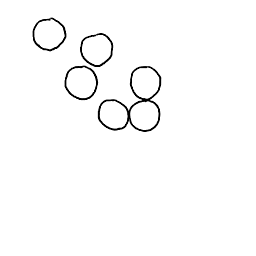
\includegraphics[width = 2cm]{figures/expert-18.png}};
  \node[draw,blue,thick,anchor = west,inner sep=0pt,minimum width = 2cm,minimum height = 2cm,label=below:Canvas: render$(S)$] (canvas) at (0,-4) {};
  \draw[lightgray,ultra thin,step = 0.125] ([xshift = 0.5,yshift = 0.5]canvas.south west) grid ([xshift = -0.5,yshift = -0.5]canvas.north east);
  % draw partial image on canvas
  \draw (0.375cm,-3.25cm) circle (0.125cm);
  \draw (0.625cm,-3.625) circle (0.125cm);
  \draw (0.75cm,-3.375) circle (0.125cm);

  \node[draw,ultra thick,anchor = west,inner sep=0pt,minimum width = 2cm,minimum height = 3cm] (CNN) at (4.5,-2.5) {CNN};
  \node[inner sep = 0pt](tensorProduct) at ([xshift = -1.5cm]CNN.west) {$\bigoplus$};

  \node[rotate = -90,draw,ultra thick,inner sep=0pt,minimum width = 3cm,minimum height = 0.5cm] (features) at ([xshift = 1.5cm]CNN.east) {Image features};

  \node[draw,ultra thick,minimum size = 1cm](c1) at ([xshift = 1.5cm]features.north) {MLP};
  \node(l1) at ([yshift = -1.5cm]c1.south) {\verb|circle(|};
  \node[draw,ultra thick,minimum size = 1cm](a2) at ([xshift = 1cm,yshift = 1.5cm]c1.east) {STN};
  \node[draw,ultra thick,minimum size = 1cm](c2) at ([xshift = 1cm]c1.east) {MLP};
  \draw[->,ultra thick] (a2.south) -- (c2.north);
  \draw[->,ultra thick,red] (c1.south) -- (l1.north);
  \node(l2) at ([yshift = -1.5cm]c2.south) {\verb|X=7,|};
  \draw[->,ultra thick,red] (c2.south) -- (l2.north);
  \node[draw,ultra thick,minimum size = 1cm](a3) at ([xshift = 1cm,yshift = 1.5cm]c2.east) {STN};
  \node[draw,ultra thick,minimum size = 1cm](c3) at ([xshift = 1cm]c2.east) {MLP};
  
  \draw[->,ultra thick] (a3.south) -- (c3.north);
  \node(l3) at ([yshift = -1.5cm]c3.south) {\verb|Y=12)|};
  \draw[->,ultra thick,red] (c3.south) -- (l3.north);

  
  \draw[->,ultra thick] (features.north) -- (c1.west);
  \draw[->,ultra thick] (features.north) to[out = 45,in = 160] (a2.north);
  \draw[->,ultra thick] (features.north) to[out = 70,in = 140] (a3.north);
  \draw[->,ultra thick] ([xshift = 0.25cm]l1.north) -- (c2.west);
  \draw[->,ultra thick] ([xshift = 0.25cm]l1.north) -- ([yshift = -0.2cm]c3.west);
  \draw[->,ultra thick] ([xshift = 0.25cm]l2.north) -- ([yshift = -0.25cm]c3.west);

  \node(next)[draw,very thick,fit = (l1) (l2) (l3), dashed, label = below:{Next drawing command}] {};

  \draw[-{>[scale = 1.5]},very thick,dashed] (next.west) -- ([yshift = -0.2cm]canvas.east) node [midway, below, sloped] (TextNode) {Renderer}; %: \LaTeX~Ti\emph{k}Z};
  
  \draw[->,ultra thick] (canvas.east) -- (tensorProduct.south);%[yshift = -0.5cm]CNN.west);
  \draw[->,ultra thick] (observation.east) -- (tensorProduct.north);%([yshift = 0.5cm]CNN.west);
  \draw[->,ultra thick] (tensorProduct.east)  -- node[fill = white,rotate = 90] {{\tiny $256\times 256\times 2$}}  (CNN.west);
  \draw[->,ultra thick] (CNN.east) -- node[fill = white,rotate = 90] {{\tiny $16\times 16\times 10$}} (features.south);
%  \draw[]
  
%  \node at (canvas.x,canvas.y) {Canvas};
\end{tikzpicture}
\caption{Our neural architecture for inferring the spec of a graphics program from its output. \textcolor{blue}{Blue}: network inputs. Black: network operations. \textcolor{red}{Red}: samples from a multinomial. \texttt{Typewriter font}: network outputs. Renders snapped to a $16\times 16$ grid, illustrated in \textcolor{gray}{gray}. STN (spatial transformer network) is a differentiable attention mechanism~\citep{jaderberg2015spatial}.}  \label{architecture}
\end{figure}
\subsection{Convolutional network}\label{CNNarchitecture}
The convolutional network takes as input 2 $256\times 256$ images
represented as a $2\times 256\times 256$ volume. These are
passed through two layers of convolutions separated by ReLU
nonlinearities and max pooling:
\begin{itemize}
\item Layer 1: 20 $8\times 8$ convolutions, 2 $16\times 4$ convolutions, 2 $4\times 16$ convolutions. Followed by $8\times 8$ pooling with a stride size of 4.
\item Layer 2: 10 $8\times 8$ convolutions. Followed by $4\times 4$ pooling with a stride size of 4.
\end{itemize}


\subsection{Autoregressive decoding of drawing commands}

Given the image features $f$, we predict the first token (i.e., the name of the drawing command: \verb|circle|, \verb|rectangle|, \verb|line|, or \verb|STOP|) using logistic regression:
\begin{equation}
  \probability [t_1]\propto \exp\left( W_{t_1}f + b_{t_1}\right)
\end{equation}
where $W_{t_1}$ is a learned weight matrix and  $b_{t_1}$ is a learned bias vector.

Given an attention mechanism $a(\cdot | \cdot)$, subsequent tokens are predicted as:
\begin{equation}
  \probability [t_n|t_{1:(n - 1)}]\propto \text{MLP}_{t_1,n}(a(f|t_{1:(n - 1)}) \oplus \bigoplus_{j < n} \text{oneHot}(t_j))\label{discreteTokenPrediction}
\end{equation}
Thus each token of each drawing primitive has its own learned MLP.
For predicting the coordinates of lines we found that using 32 hidden nodes with sigmoid activations worked well;
for other tokens the MLP's are just logistic regression (no hidden nodes).

We use Spatial Transformer Networks~\cite{jaderberg2015spatial}
as our attention mechanism.
The parameters of the spatial transform are predicted on the basis of previously predicted tokens.
For example, in order to decide where to focus our attention when predicting the $y$ coordinate of a circle,
we condition upon both the identity of the drawing command (\verb|circle|) and upon the value of the previously predicted $x$ coordinate:
\begin{equation}
  a(f|t_{1:(n - 1)}) = \text{AffineTransform}(f, \text{MLP}_{t_1,n}(\bigoplus_{j < n}\text{oneHot}(t_j)))
  \label{spatialTransformEquation}
\end{equation}
So, we learn a different network for predicting special transforms
\emph{for each drawing command} (value of $t_1$) and also \emph{for each token of the drawing command}.
These networks ($\text{MLP}_{t_1,n}$ in equation~\ref{spatialTransformEquation}) have no hidden layers and
output the 6 entries of an affine transformation matrix; see~\cite{jaderberg2015spatial}
for more details.

Training takes a little bit less than a day on a Nvidia TitanX GPU.
The network was trained on $10^5$ synthetic examples.
\subsection{LSTM Baseline}

We  compared our deep network with a baseline that models the problem as a kind of image captioning.
Given the target image, this baseline produces the program spec in one shot by
using a CNN to extract features of the input which are passed to an LSTM which finally predicts
the spec token-by-token.
This general architecture is used in several successful neural models of image captioning (e.g.,~\cite{vinyals2015show}).

Concretely, we kept the image feature extractor architecture (a CNN) as in our model,
but only passed it one image as input (the target image to explain).
Then, instead of using an autoregressive decoder to predict a single drawing command,
we used an LSTM to predict a sequence of drawing commands token-by-token.
This LSTM had 128 memory cells,
and at each time step produced as output the next token in the sequence of drawing commands.
It took as input both the image representation and its previously predicted token.

\subsection{Generating synthetic training data}

We generated synthetic training data for the neural network by
sampling \LaTeX~code according to the following generative process:
First,
the number of objects in the scene are sampled uniformly from 1 to 12.
For each object we uniformly sample its identity (circle, rectangle, or line).
Then we sample the parameters of the circles,
than the parameters of the rectangles,
and finally the parameters of the lines;
this has the effect of teaching the network to first draw the circles in the scene,
then the rectangles,
and finally the lines.
We furthermore put the circle (respectively, rectangle and line) drawing commands in order by
left-to-right, bottom-to-top;
thus the training data enforces a canonical order in which to draw any scene.

To make the training data look more like naturally occurring figures,
we put a Chinese restaurant process prior~\cite{gershman2012tutorial} over
the values of the X and Y coordinates that occur in the execution spec.
This encourages reuse of coordinate values,
and so produces training data that tends to have parts that are nicely aligned.

In the synthetic training data we excluded any sampled scenes that had
overlapping drawing commands.  As shown in the main paper, the network
is then able to generalize to scenes with, for example, intersecting
lines or lines that penetrate a rectangle.

When sampling the endpoints of a line,
we biased the sampling process so that it would
be more likely to start an endpoint
along one of the sides of a rectangle or at the boundary of a circle.
If $n$ is the number of points either along the side of a rectangle or at the boundary of a circle,
we would sample an arbitrary endpoint with probability $\frac{2}{2 + n}$
and sample one of the ``attaching'' endpoints with probability $\frac{1}{2 + n}$.

See figure~\ref{exampleTrainingData} for examples of the kinds of scenes that the network is trained on.
\begin{figure}
  \begin{minipage}[t]{2.2cm}\fbox{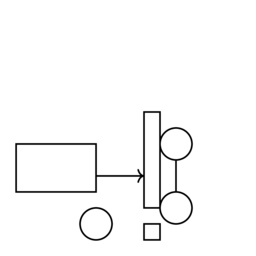
\includegraphics[width=2cm]{figures/randomScene-58-7.png}}\end{minipage}
  \begin{minipage}[t]{2.2cm}\fbox{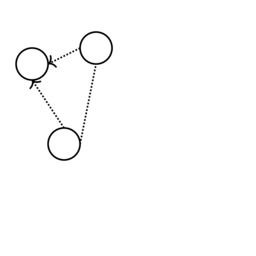
\includegraphics[width=2cm]{figures/randomScene-33-5.png}}\end{minipage}
  \begin{minipage}[t]{2.2cm}\fbox{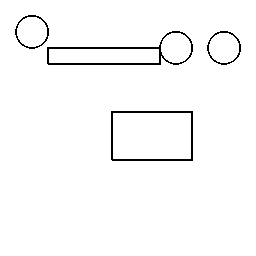
\includegraphics[width=2cm]{figures/randomScene-4-4.png}}\end{minipage}
  \begin{minipage}[t]{2.2cm}\fbox{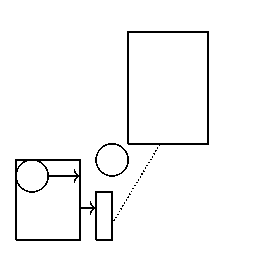
\includegraphics[width=2cm]{figures/randomScene-26-7.png}}\end{minipage}
      \begin{minipage}[t]{2.2cm}\fbox{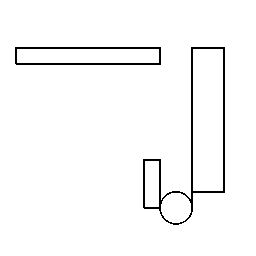
\includegraphics[width=2cm]{figures/randomScene-25-4.png}}\end{minipage}\\
      \begin{minipage}[t]{2.2cm}\fbox{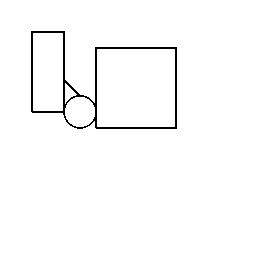
\includegraphics[width=2cm]{figures/randomScene-22-3.png}}\end{minipage}
      \begin{minipage}[t]{2.2cm}\fbox{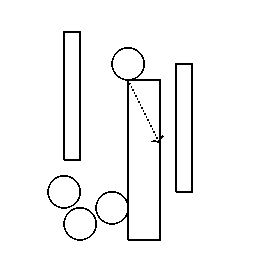
\includegraphics[width=2cm]{figures/randomScene-20-7.png}}\end{minipage}
      \begin{minipage}[t]{2.2cm}\fbox{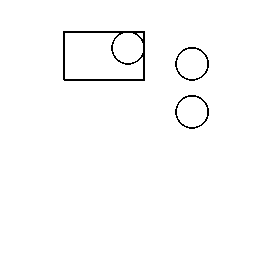
\includegraphics[width=2cm]{figures/randomScene-19-3.png}}\end{minipage}
      \begin{minipage}[t]{2.2cm}\fbox{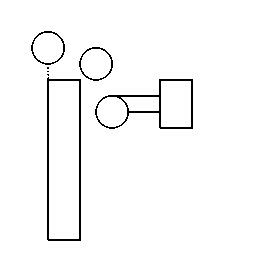
\includegraphics[width=2cm]{figures/randomScene-17-7.png}}\end{minipage}
      \begin{minipage}[t]{2.2cm}\fbox{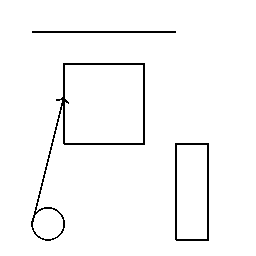
\includegraphics[width=2cm]{figures/randomScene-1-4.png}}\end{minipage}
      \caption{Example synthetic training data}\label{exampleTrainingData}
\end{figure}

For readers wishing to generate their own synthetic training sets,
we refer them to our source code at:~\url{https://github.com/ellisk42/TikZ}.


%\pagebreak
\section{Generalizing to real hand drawings}
\subsection{Simulating hand drawings}\label{simulatingHandDrawings}

We introduce noise into the \LaTeX~rendering process by:

\begin{itemize}
\item Rescaling the image intensity by a factor chosen uniformly at random from $[0.5,1.5]$
\item Translating the image by $\pm 3$ pixels chosen uniformly random
\item Rendering the \LaTeX~using the \verb|pencildraw| style,
  which adds random perturbations to the paths drawn by \LaTeX in a way designed to resemble a pencil.
\item Randomly perturbing the positions and sizes of primitive  \LaTeX drawing commands
\end{itemize}

\begin{figure}
  
  
\centering\vspace{-0.7cm}  \begin{minipage}[t]{2.5cm}\centering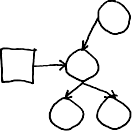
\includegraphics[width = 2cm]{figures/expert-60-reduced.png}
    \subcaption{hand drawing}
  \end{minipage}\\
   \begin{minipage}[t]{2.5cm}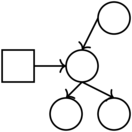
\includegraphics[width = 2cm]{figures/60-groundTruth-reduced.png}
    \subcaption{rendering of (a)'s inferred spec}
  \end{minipage}\qquad% 
  \begin{minipage}[t]{2.5cm}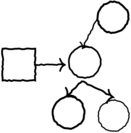
\includegraphics[width = 2cm]{figures/60-1-reduced.png}
    \subcaption{noisy rendering of (b)}
  \end{minipage}%
  \caption{Noisy renderings produced in \LaTeX~Ti\emph{k}Z w/ \texttt{pencildraw} package }
    \label{handDrawingExamples} 
\end{figure}

\subsection{A learned likelihood surrogate}

Our architecture for
$L_{\text{learned}}(\text{render}(T_1)|\text{render}(T_2))$ has the
same series of convolutions as the network that predicts the next
drawing command. We train it to predict two scalars: $|T_1 - T_2|$ and
$|T_2 - T_1|$.  These predictions are made using linear regression
from the image features followed by a ReLU nonlinearity; this
nonlinearity makes sense because the predictions can never be negative
but could be arbitrarily large positive numbers.

We train this network by sampling random synthetic scenes for $T_1$,
and then perturbing them in small ways to produce $T_2$.
We minimize the squared loss between the network's prediction and the ground truth symmetric differences.
$T_1$ is rendered in a ``simulated hand drawing'' style which Section~\ref{simulatingHandDrawings} describes.
%\pagebreak

\section{The cost function for programs}

We seek the minimum cost program which evaluates to (produces the drawing primitives in) an execution spec $T$:
\begin{equation}
  \text{program}(T) = \argmin_{\substack{p\in \text{DSL}\\p \text{ evaluates to } T}} \text{cost}(p)\label{programObjective}
\end{equation}

Programs incur a cost of 1 for each command (primitive drawing action,
loop, or reflection).  They incur a cost of $\frac{1}{3}$ for each
unique coefficient they use in a linear transformation beyond the
first coefficient. This encourages reuse of coefficients, which leads
to code that has translational symmetry; rather than provide a
translational symmetry operator as we did with reflection, we modify
what is effectively a prior over the space of program so that it tends
to produce programs that have this symmetry.

Programs also incur a cost of 1 for having loops of constant length 2;
otherwise there is often no pressure from the cost function to explain
a repetition of length 2 as being a reflection rather a loop.


\section{Learning a search policy}
\subsection{Modeling}\label{searchPolicyModel}
Recall from the main paper that our goal is to estimate the policy minimizing the following loss:
\begin{align}
\textsc{Loss}(\theta ; \mathcal{D})& =  \expect_{S\sim\mathcal{D}}\left[ \min_{\sigma\in \text{\textsc{Best}}(S)}\frac{t(\sigma | S)}{\pi_\theta (\sigma | S)}\right] + \lambda \Vert\theta\Vert_2^2\label{policyLoss}\\
\text{where }  \sigma \in\text{\textsc{Best}}(S) &\text{ if  a minimum cost program for }S \text{ is in }\sigma .\nonumber %\text{cost}(\text{program}(p)) = \min_{p\in \sigma \text{, s.t. }p\text{ evaluates to }S} \text{cost}(p) \nonumber
\end{align}
We make this optimization problem tractable by annealing our loss function during gradient descent:
\begin{align}
&  \textsc{Loss}_\beta(\theta ; \mathcal{D}) =  \expect_{S\sim\mathcal{D}}\left[ \textsc{SoftMinimum}_\beta \left\{
    \frac{t(\sigma | S)}{\pi_\theta (\sigma | S)}    : \sigma\in \text{\textsc{Best}}(S)\right\}\right] + \lambda \Vert\theta\Vert_2^2\label{softenedObjective}\\
  \text{where }&\textsc{SoftMinimum}_\beta (x_1,x_2,x_3,\cdots ) = \sum_n x_n  \frac{e^{-\beta x_n}}{\sum_{n'}e^{-\beta x_{n'}}}
\end{align}
Notice that $\textsc{SoftMinimum}_{\beta = \infty}(\cdot )$ is just $\min(\cdot )$.
We set the regularization coefficient $\lambda = 0.1$ and minimize equation~\ref{softenedObjective}
using Adam for 2000 steps, linearly increasing $\beta$ from $1$ to $2$.

We parameterize the space of policies as a simple log bilinear model:
\begin{equation}
  \pi_{\theta}(\sigma |S)\propto \exp \left( \phi_{\text{params}}(\sigma )^\top\theta \phi_{\text{spec}}(S)\right)
\end{equation}
where:
\begin{align*}
  \phi_{\text{params}}(\sigma ) = [&\indicator [\sigma \text{ can loop}] ;\\
    &\indicator [\sigma \text{ can reflect}];\\
    &\indicator [\sigma \text{ is incremental}] ; \\
    &\indicator [\sigma \text{ has depth bound }1];\indicator [\sigma \text{ has depth bound }2];\indicator [\sigma \text{ has depth bound }3];]\\
  \phi_{\text{spec}}(S) = [&\text{\# circles in }S;\text{\# rectangles in }S;\text{\# lines in }S;1]
  \end{align*}
where the meaning of ``incremental'' is described in the next section.
\subsection{Incremental Solving}
Rather than give the sketch program synthesizer the entire spec all at once,
we can instead give it subsets of the spec (subsets of the objects in the image)
and ask it to synthesize a program for each subset.
We then concatenate the resulting programs from each subset to get a program that explains the entire image,
and we call this strategy ``incremental solving''.
Incremental solving is not guaranteed to be faster,
nor is it guaranteed to find a minimum cost program.
Thus we allow the search policy to decide
what fraction of our search time should be allocated to this incremental approach to program synthesis.
Concretely, we partitioned a spec into its constituent lines, circles, and rectangles.
\subsection{Baseline comparisons}

\subsubsection{DeepCoder-style baseline}

In addition to the end-to-end baseline,
we compared with a DeepCoder-style baseline (main paper, Section 3.1).
DeepCoder (DC)~\cite{BalGauBroetal16}
is an approach for learning to speed up program synthesizers.
DC models are neural networks that
predict, starting from a spec,
the probability of a DSL component being in a minimal-cost program satisfying the spec.
Writing $\text{DC}(S)$ for the distribution predicted by the neural network,
DC is trained to maximize  the following objective:
\begin{equation}
  \expect_{S\sim\mathcal{D}}\left[\min_{p\in \text{\textsc{Best}}(S)} \sum_{x\in \text{DSL}} \log \left(\indicator\left[x\in p \right] \text{DC}(S)_x + \indicator\left[x\notin p \right] (1 - \text{DC}(S)_x)\right)
    \right]
\end{equation}
where $x$ ranges over DSL components and $\text{DC}(S)_x\in \left[0,1 \right]$  is the probability predicted by the DC model for component $x$ for spec $S$.

We provided our DC model with the same features given to our bias optimal search policy ($\phi_{spec}$ in section~\ref{searchPolicyModel}), and trained using the same 20-fold cross validation splits.
To evaluate the DC baseline on held out data,
we used the \emph{Sort-and-Add} policy described in the DeepCoder paper\cite{BalGauBroetal16}.


\subsubsection{End-to-End baseline}

Recall that we factored the graphics program synthesis problem into two components: (1) a perception-facing component, whose job is to go from perceptual input to a set of commands that must occur in the execution of the program (\textbf{spec}); and (2) a program synthesis component, whose job is to infer a program whose execution contains those commands. This is a different approach from other recent program induction models (e.g.,~\cite{devlin2017robustfill,nps}), which regress directly from a program induction problem to the source code of the program.

\textbf{Experiment.} To test whether this factoring is necessary for our domain, we trained a model to regress directly from images to graphics programs. This baseline model, which we call the \emph{no-spec baseline}, was able to infer some simple programs, but failed completely on more sophisticated scenes.

Baseline model architecture: The model architecture is a straightforward, image-captioning-style CNN$\to$LSTM. We keep the same CNN architecture from our main model (Section~\ref{CNNarchitecture}), with the sole difference that it takes only one image as input. The LSTM decoder produces the program token-by-token: so we flatten the program's hierarchical structure, and use special ``bracketing'' symbols to convey nesting structure, in the spirit of~\citep{vinyals2015grammar}. The LSTM decoder has 2 hidden layers with 1024 units. We used 64-dimensional embeddings for the program tokens.

Training and evaluation: The model was trained on $10^7$ synthetically generated programs -- 2 orders of magnitude more data than the model we present in the main paper. We then evaluated the baseline on \emph{synthetic renders} of our 100 hand drawings (the testing set used throughout the paper). Recall that our model was evaluated on noisy real hand drawings. We sample programs from this baseline model conditioned on a synthetic render of a hand drawing, and report only the sampled program whose output most closely matched the ground truth spec spec, as measured by the symmetric difference of the two sets. We allow the baseline model to spend 1 hour drawing samples per drawing -- recall that our model finds 58\% of programs in under a minute. Together these training and evaluation choices are intended to make the problem as easy as possible for the baseline.

Results: The no-spec baseline succeeds for trivial programs (a few lines, no variables, loops, etc.); occasionally gets small amounts of simple looping structure; and fails utterly for most of our test cases. See Figure~\ref{noSpec}.

\begin{figure}[h]\centering
      \includegraphics[width = 2cm]{figures/noTraceOutputs/11.png}
  \includegraphics[width = 2cm]{figures/noTraceOutputs/16.png}
    \includegraphics[width = 2cm]{figures/noTraceOutputs/29.png}
    \includegraphics[width = 2cm]{figures/noTraceOutputs/7.png}
        \includegraphics[width = 2cm]{figures/noTraceOutputs/94.png}
      \includegraphics[width = 2cm]{figures/noTraceOutputs/38.png}
  \caption{Top, white: synthetic rendering of a hand drawing. Bottom, black: output of best program found by no-spec baseline.}\label{noSpec}
  \end{figure}
 

\section{Correcting errors made by the neural network}\label{synthesizerHelpsParsing}
The program synthesizer can help correct errors from the execution spec proposal network by favoring execution specs which lead to more concise or general programs.
For example, one generally prefers figures with perfectly aligned objects over figures whose parts are slightly misaligned -- and precise alignment lends itself to short programs.
Similarly, figures often have repeated parts,
which the program synthesizer might be able to model as a loop or reflectional symmetry.
So, in considering several candidate specs proposed by the neural network,
we might prefer specs whose best programs have desirable features such being short or having iterated structures.

Concretely, we implemented the following scheme: for an image $I$, the neurally guided sampling scheme of section 2 of the main paper samples a set of candidate specs, written $\mathcal{F}(I)$.
Instead of predicting the most likely spec in $\mathcal{F}(I)$ according to the neural network,
we can take into account the programs that best explain the specs. 
Writing $\hat{S}(I)$ for the spec the model predicts for image $I$,
\begin{equation}
\hat{S}(I) = \argmax_{S\in \mathcal{F}(I)} L_{\text{learned}}(I | \text{render}(S))\times \probability_\theta[S|I] \times\probability_{\beta} [ \text{program}(S)] 
\end{equation}
where $\probability_{\beta} [\cdot]$ is a prior probability
distribution over programs parameterized by $\beta$.
This is equivalent to doing
MAP inference in a generative model where the program is first drawn
from $\probability_{\beta} [\cdot]$, then the program is executed deterministically,
and then we observe a noisy version of the program's output, where $L_\text{learned}(I|\text{render}(\cdot))\times\probability_\theta[\cdot|I]$
is our observation model.

Given a corpus of graphics program synthesis problems with annotated ground truth specs (i.e. $(I,S)$ pairs),
we find a maximum likelihood estimate of $\beta$:
\begin{equation}
  \beta^* = \argmax_{\beta} \expect \left[ \log \frac{\probability_{\beta} [\text{program}(S)]\times L_{\text{learned}}(I|\text{render}(S))\times \probability_\theta[S|I]}{\sum_{S'\in \mathcal{F}(I)} \probability_{\beta} [\text{program}(S')]\times L_{\text{learned}}(I|\text{render}(S'))\times \probability_\theta[S'|I]} \right]
\end{equation}
where the expectation is taken both over the model predictions and the
$(I,S)$ pairs in the training corpus.  We define $\probability_{\beta}
[\cdot]$ to be a log linear distribution $\propto \exp
(\beta\cdot \phi(\text{program}))$, where $\phi(\cdot)$ is a feature
extractor for programs.  We extract a few basic features of a
program, such as its size and how many loops it has, and use these
features to help predict whether a spec is the correct explanation
for an image.

We synthesized programs for the top 10 specs
output by the deep network.  Learning this prior over programs can
help correct mistakes made by the neural network, and also
occasionally introduces mistakes of its own; see
Fig.~\ref{exampleOfProgramCorrectingMistake} for a representative
example of the kinds of corrections that it makes. On the whole
it modestly improves our Top-1 accuracy from 63\% to 67\%.  Recall that
from Fig. 6 of the main paper that the best improvement
in accuracy we could possibly get is 70\% by looking at the top 10 specs. 
\begin{figure}[h]\centering
  \begin{minipage}{6cm}
      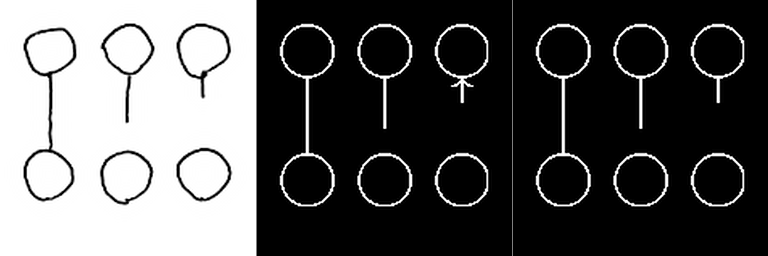
\includegraphics[width = 5cm]{figures/programSuccess7.png}
  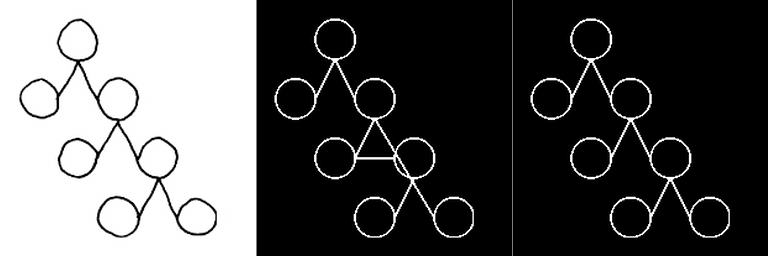
\includegraphics[width = 5cm]{figures/programSuccess16.png}
    \end{minipage}
  \caption{Left: hand drawing. Center: interpretation favored by the deep network. Right: interpretation favored after learning a prior over programs. Our learned prior favors shorter, simpler programs, thus (top example) continuing the pattern of not having an arrow is preferred, or (bottom example) continuing the binary search tree is preferred.}\label{exampleOfProgramCorrectingMistake}
\end{figure}
%\pagebreak

\section{Measuring similarity between drawings}

We measure the similarity between two drawings by extracting features
of the best programs that describe them. Our features are counts of the number of times that different components in the
DSL were used.  We project these features down to a
2-dimensional subspace using primary component analysis
(PCA); see Fig.\ref{NMF}.  One could use many
alternative similarity metrics between drawings which would capture pixel-level similarities while missing high-level geometric similarities.
We used our learned distance metric between specs, $L_{\text{learned}}(\cdot|\cdot)$, and projected to a 2-dimensional subspace using multidimensional scaling (MDS:~\cite{cox2008multidimensional}). This reveals similarities between the objects in the drawings,
while missing similarities at the level of the program.
\begin{figure}[h]
\centering  \begin{minipage}{\textwidth}\centering
  %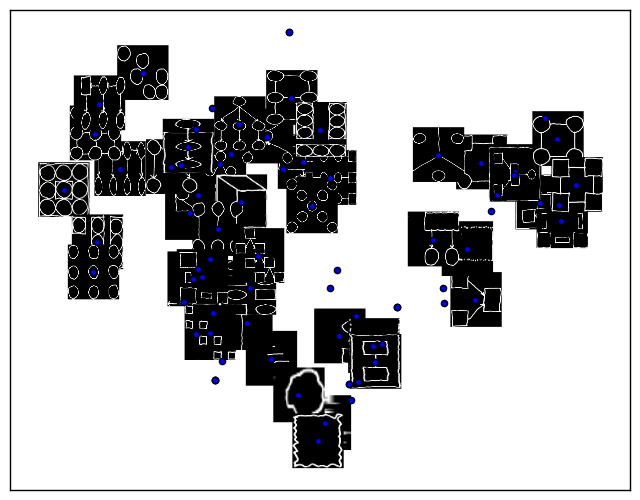
\includegraphics[width = 0.69\textwidth]{figures/PCA.png}
  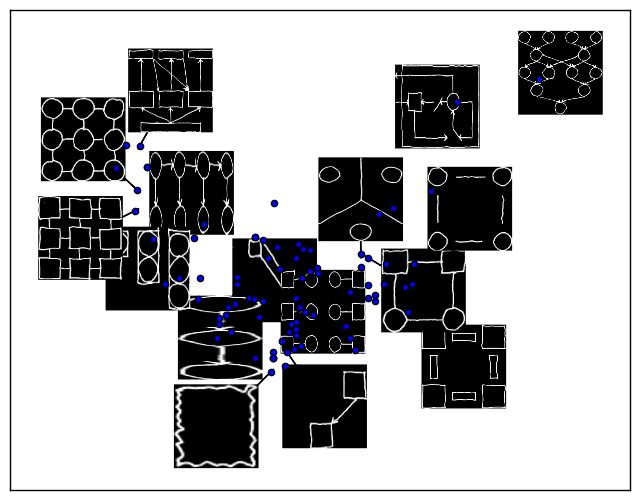
\includegraphics[width = 0.69\textwidth]{figures/PCA_improved.png}
    \caption{PCA on features of the programs that were synthesized for each drawing. Symmetric figures cluster to the right; ``loopy'' figures cluster to the left; complicated programs are at the top and simple programs are at the bottom.}    \label{NMF}
  \end{minipage} %\hfill
  \begin{minipage}{\textwidth}\centering
    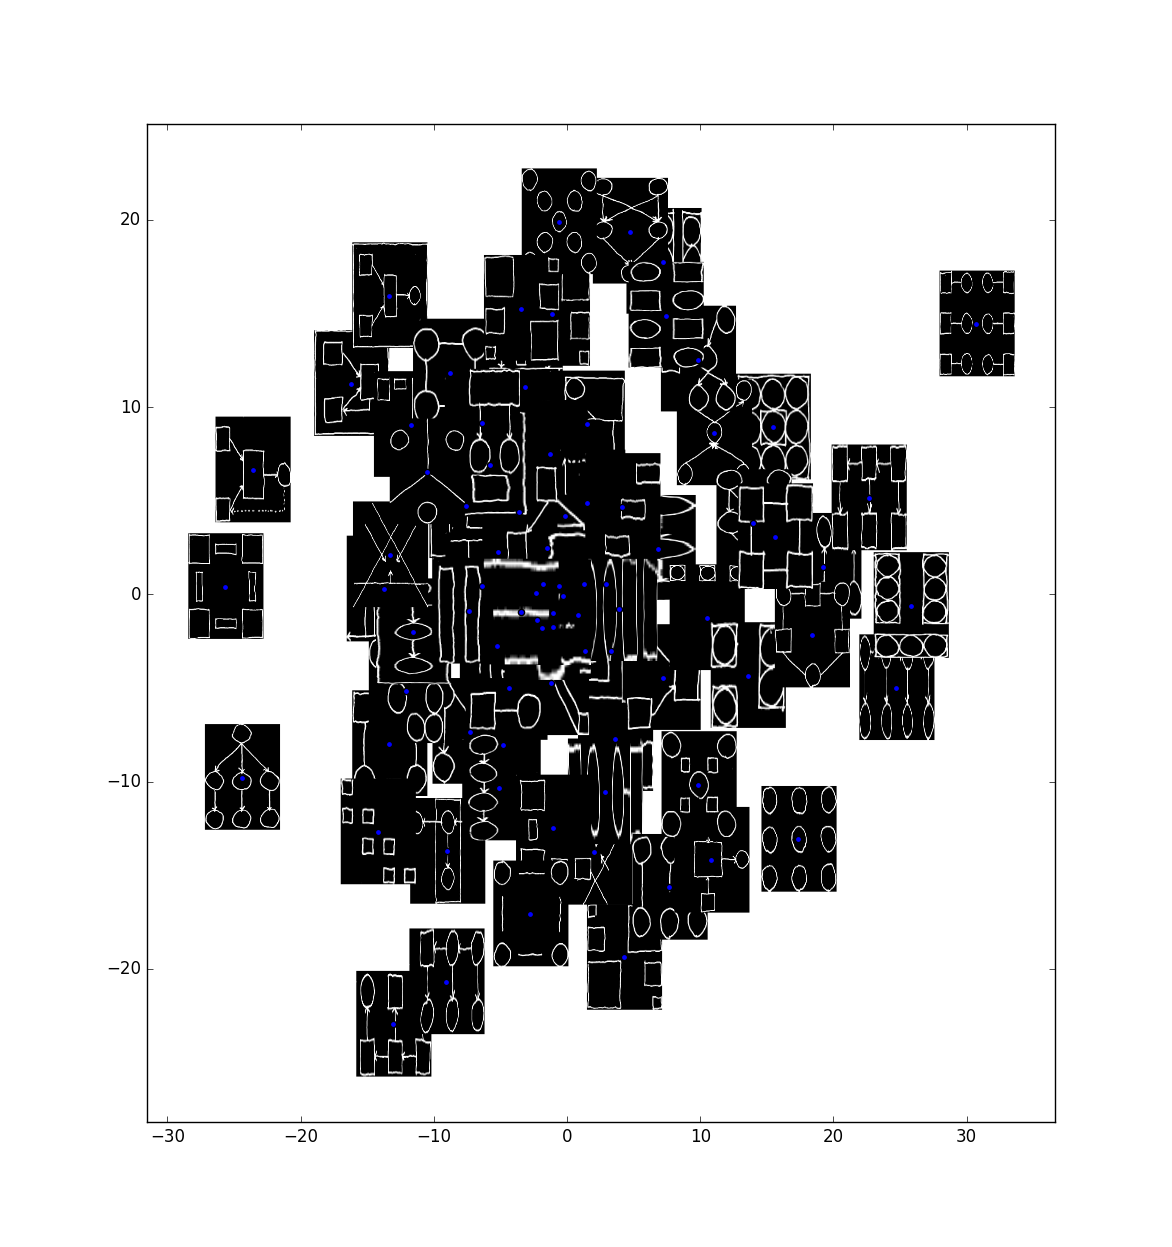
\includegraphics[width = 0.69\textwidth]{figures/imageSimilarity.png} 
    \caption{MDS on drawings using the learned distance metric, $L_{\text{learned}}(\cdot|\cdot)$. Drawings with similar looking parts in similar locations are clustered together.}
  \end{minipage}
\end{figure}





%\pagebreak

%% \begin{comment}
%% \subsection{Predicting continuous coordinates using Mixture Density Networks}

%% Our main paper describes a neural model for parsing hand drawings
%% into~\LaTeX, but comes with the restriction that all of the
%% coordinates of all the drawing commands are snapped to a $16\times 16$
%% grid. Now we describe a variant of our model that
%% can predict continuous real valued coordinates.

%% The key obstacle to overcome is \emph{multimodality}: if the network
%% is unsure whether it should predict a coordinate value of $a$ or $b$,
%% we wish to predict a distribution that splits its mass between $a$ and
%% $b$, rather than predicting the single value $\frac{a + b}{2}$.  In
%% the model where everything is snapped to a discrete grid, supporting
%% this multimodality falls out naturally from our parameterization of
%% the network predictions (i.e., the network predicts the parameters of
%% a multinomial distribution). To predict continuous real valued
%% coordinates we turn to Mixture Density Networks (MDN:~\cite{MDN}).  In
%% an MDN, a distribution over a real-valued random variable is
%% parameterized using a mixture of Gaussians, and the deep network
%% predicts the parameters of the Gaussian mixture.

%% Concretely,
%% we modify our autoregressive drawing command decoder to
%% predict distributions over real-valued coordinates
%% as:
%% \begin{equation}
%%   p(t_n|t_{1:(n - 1)}) = \text{MDN}_{t_1,n} (a(f|t_{1:(n - 1)}) \oplus \bigoplus_{j < n} t_j)\text{, if }n^{\text{th}}\text{ token is continuous}\label{continuousDensityEquation}
%% \end{equation}
%% Compare this equation with Equation~\ref{discreteTokenPrediction} to see that we have only
%% replaced a draw from a multinomial (whose parameters are predicted by an MLP)
%% with a draw from a mixture of Gaussians (whose parameters are predicted by an MDN).
%% Otherwise the two models are identical.

%% For an MDN $i$ with $K$ mixture components that takes as input $x$, we parameterize it's output distribution as:
%% \begin{eqnarray}
%%   \text{MDN}_i(x) &=& \sum_{1\leq k\leq K} \pi_{i,k}(x)\times \mathcal{N}(\mu_{i,k}(x),\sigma^2_{i,k}(x))\\
%%   \mu_{i,k}(x)& = &\text{sigmoid} (W^{\mu_{i,k}}x + b^{\mu_{i,k}}x)\label{mixtureMean}
%%   \\\sigma^2_{i,k}(x)& = &\log \left(1 + \exp\left(W^{\sigma^2_{i,k}}x + b^{\sigma^2_{i,k}}x\right) \right)
%%   \\\pi_{i,k}(x)& = &\frac{\exp\left(W^{\pi_{i,k}}x + b^{\pi_{i,k}}x \right)}{\sum_{k'} \exp\left(W^{\pi_{i,k'}}x + b^{\pi_{i,k'}}x \right)}
%%   \end{eqnarray}
%% where $W$ with a superscript is a learned weight matrix and $b$ is a
%% learned bias vector. Notice that Equation~\ref{mixtureMean} normalizes
%% the predicted means to be within $[0,1]$: this is because we wish to
%% constrain the predicted coordinates to lie within the plane
%% $[0,1]^2$. We used $K = 16$ mixture components.

%% Figure~\ref{syntheticContinuous}  shows the behavior of the MDN variant of our model on noisy synthetic drawings.
%% Contrast these mediocre results with Figure~4 of the main paper to see that although
%% our main model is essentially at ceiling for parsing scenes like these,
%% the MDN variant fares poorly in comparison.
%% \begin{figure}
%%   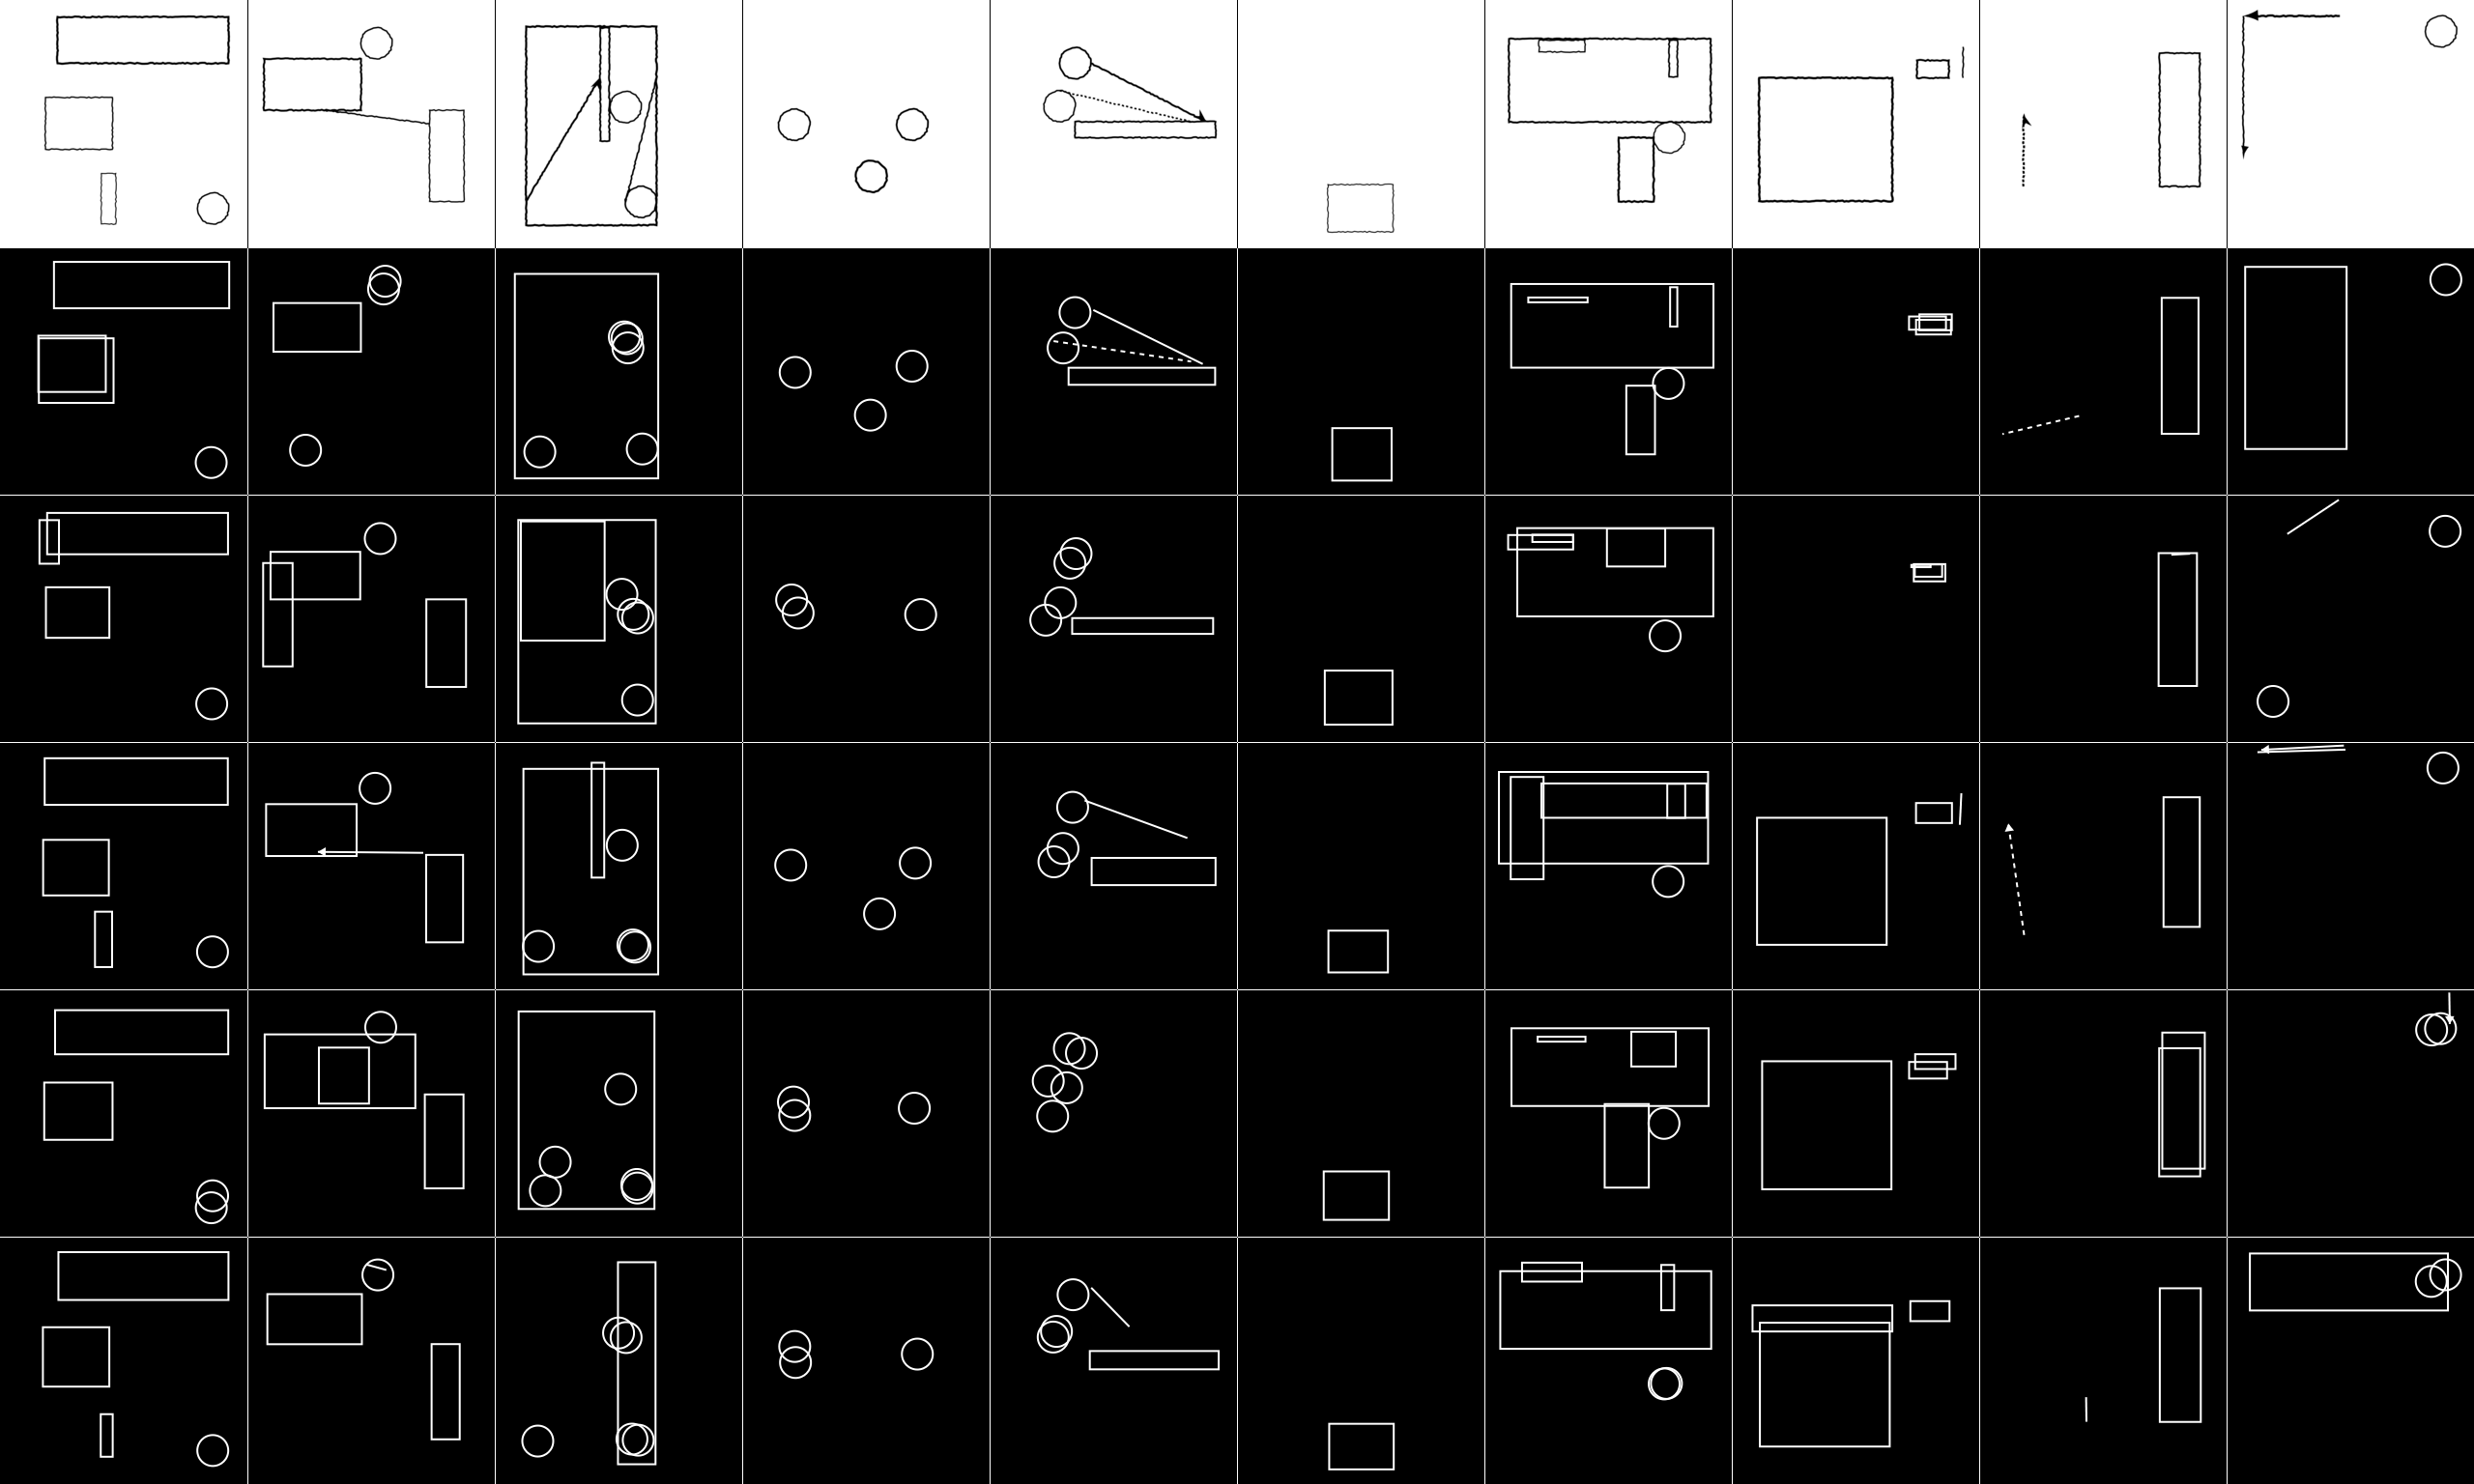
\includegraphics[width = \textwidth]{figures/syntheticContinuous.png}
%%   \caption{Left column: \LaTeX~output corrupted by noise process designed to resemble the variability is introduced by hand drawings. Right columns: samples from the MDN variant of the model.}\label{syntheticContinuous}
%% \end{figure}

%% We evaluated the MDN version of our model on hand drawings by (1)
%% performing a beam search in order to find the spec maximizing
%% $\probability [T|I]$, and (2) constraining the predicted coordinates
%% to lie on the $16\times 16$ grid. We constrain the predicted coordinates
%% to lie on the grid by integrating the predicted densities about each grid location.
%% So, using the probability density $p(t_n|t_{1:(n - 1)})$ in Eq.~\ref{continuousDensityEquation},
%% we compute a probability mass function $\probability [t_n|t_{1:(n - 1)}]$ as:
%% \begin{equation}
%%   \probability [t_n = t|t_{1:(n - 1)}] = \int_{t - \frac{1}{2}}^{t + \frac{1}{2}} \mathrm{d}t_n \; p(t_n|t_{1:(n - 1)})\label{constrainingEquation}
%% \end{equation}
%% Even after using Eq.~\ref{constrainingEquation} to constrain the predicted coordinates to lie on the $16\times 16$ grid, the MDN variant of the model only produces finished specs for 48/100 of the drawings.
%% See Figure~\ref{continuousParses} to see the specs recovered by the beam search.

%% \begin{figure}
%%   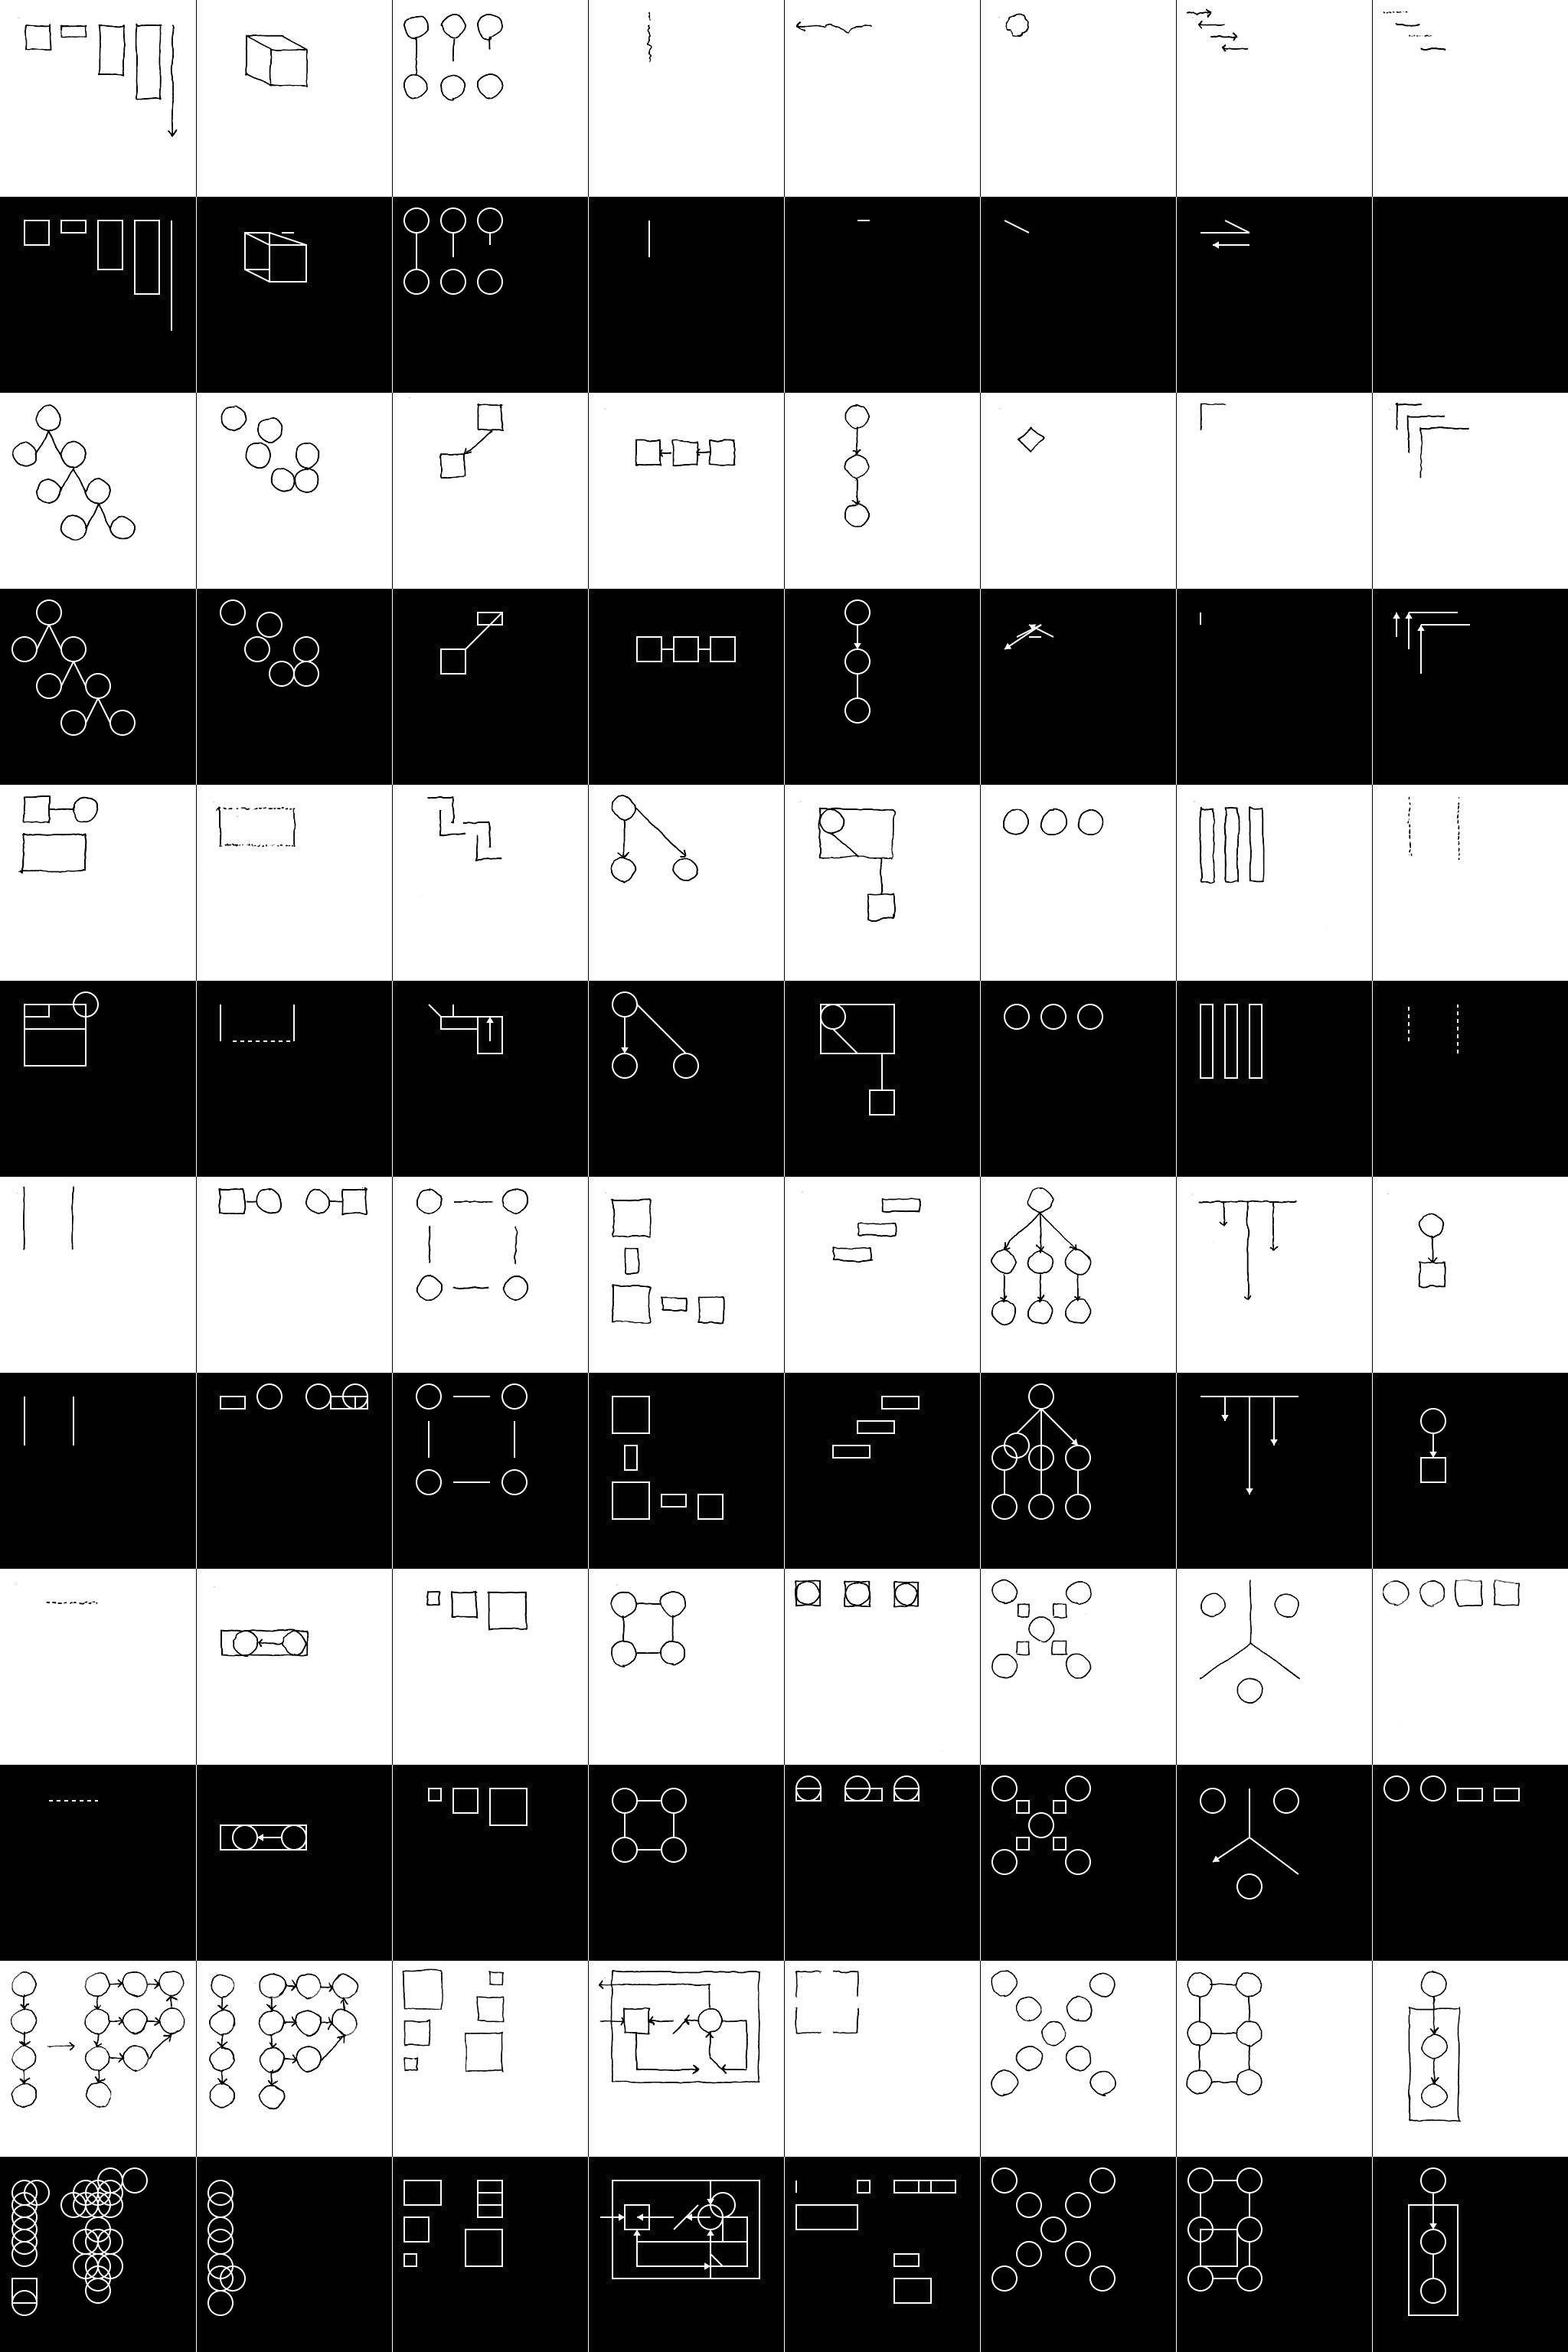
\includegraphics[width = \textwidth]{figures/continuousParses.png}
%%   \caption{Parsing hand drawings using the MDN variant of our
%%     model. Black-on-white: hand drawings. White-on-black, below each
%%     hand drawing: the parse inferred by the model.}\label{continuousParses} 
%%   \end{figure}
%% \end{comment}



%% \section{Neural networks for guiding SMC}



%% Let $L(\cdot | \cdot):\text{image}^2\to \mathcal{R}$ be our likelihood
%% function: it takes two images, an observed target image and a
%% hypothesized program output, and gives the likelihood of the observed
%% image conditioned on the program output. We want to sample from:
%% \begin{equation}
%% \probability [p|x]  \propto L(x | \text{render}(p)) \probability [p]
%% \end{equation}
%% where $\probability [p]$ is the prior probability of program $p$, and $x$ is the observed image.

%% Let $p$ be a program with $L$ lines, which we will write as $p = (p_1,p_2,\cdots,p_L)$. Assume the prior factors into:
%% \begin{equation}
%%   \probability [p]\propto \prod_{l\leq L}\probability [p_l]
%% \end{equation}
%% Define the distribution $q_L(\cdot)$, which happens to be proportional to the above posterior:
%% \begin{equation}
%%   q_L(p_1,p_2,\cdots,p_{L - 1},p_L)\propto q_{L - 1}(p_1,p_2,\cdots,p_{L - 1})\times \frac{L(x | \text{render}(p_1,p_2,\cdots,p_{L - 1},p_L))}{L(x | \text{render}(p_1,p_2,\cdots,p_{L - 1}))}\times\probability [p_L]
%% \end{equation}
%% Now suppose we have some samples from $q_{L - 1}(\cdot)$, and that we
%% then sample a $p_L$ from a distribution proportional to $\frac{L(x |
%%   \text{render}(p_1,p_2,\cdots,p_{L - 1},p_L))}{L(x |
%%   \text{render}(p_1,p_2,\cdots,p_{L - 1}))}\times\probability [p_L]$.
%% The resulting programs $p$ are distributed according to $q_L$, and so
%% are also distributed according to $\probability [p|x]$.

%% How do we sample $p_L$ from a distribution proportional to $\frac{L(x
%%   | \text{render}(p_1,p_2,\cdots,p_{L - 1},p_L))}{L(x |
%%   \text{render}(p_1,p_2,\cdots,p_{L - 1}))}\times\probability [p_L]$?
%% We have a neural network that takes as input the target image $x$ and
%% the program so far, and produces a distribution over next lines of
%% code ($p_L$).  We write $\text{NN}(p_L | p_1,\cdots,p_{L - 1};x)$ for
%% the distribution output by the neural network. So we can sample from NN and then weight the samples by:
%% \begin{equation}
%%   w(p_L) = \frac{\probability [p_L]}{\text{NN}(p_L | p_1,\cdots,p_{L - 1};x)}\times \frac{L(x | \text{render}(p_1,p_2,\cdots,p_{L - 1},p_L))}{L(x | \text{render}(p_1,p_2,\cdots,p_{L - 1}))}
%% \end{equation}
%% Then we can resample from these now weighted samples to get a new
%% population of particles (here programs are particles), where each
%% program now has $L$ lines instead of $L - 1$.

%% This procedure can be seen as a particle filter, where each successive
%% latent variable is another line of code, and the emission
%% probabilities are successive ratios of likelihoods under $L(\cdot |
%% \cdot)$.


%%   \begin{algorithm}[tb]
%%    \caption{Neurally guided SMC}
%%    \label{guideAlgorithm}
%% \begin{algorithmic}
%%   \STATE {\bfseries Input:} Neural network NN, beam size $N$, maximum length $L$, target image $x$
%%   \STATE {\bfseries Output:} Samples of the program spec
%%   \STATE Set $B_0 = \{\text{empty program}\}$
%%   \FOR{$1\leq l\leq L$}
%%   \FOR{$1\leq n\leq N$}
%%   \STATE{ $p_n\sim \text{Uniform}(B_{l - 1})$}
%%   \STATE{ $p'_{n}\sim \text{NN}(\text{render}(p),x)$}
%%   \STATE{ Define $r_n = p'_n\cdot p_n$}
%%   \STATE{ Set $\tilde{w}(r_n) = \frac{L(x|r_n)}{L(x|p_n)}\times\frac{\probability [p'_n]}{\probability [p'_n = \text{NN}(\text{render}(p),x)]}$}
%%   \ENDFOR
%%   \STATE{ Define $w(p) = \frac{\tilde{w}(p)}{\sum_{p'}\tilde{w}(p')}$}
%%   \STATE{ Set $B_l$ to be $N$ samples from $r_n$ distributed according to $w(\cdot)$}
%%   \ENDFOR
%%   \STATE {\bfseries return} $\{p : p\in B_{l\leq L}, p \text{ is finished}\}$
%% \end{algorithmic}
%%   \end{algorithm}

\section{Full results on drawings data set}

Below we show our full data set of drawings. The leftmost column is a hand drawing. The middle column is a rendering of the most likely spec discovered by the neurally guided SMC sampling scheme. The rightmost column is the program we synthesized from a ground truth execution spec of the drawing.
Note that because the inference procedure is stochastic,
the top one most likely sample can vary from run to run.
Below we report a representative sample from a run with 2000 particles.

            \begin{tabular}{lll}
    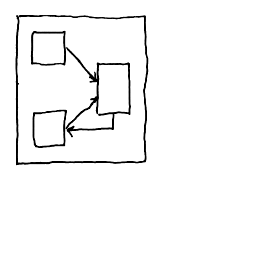
\includegraphics[width = 5cm]{../TikZ/drawings/expert-0.png}&
            \includegraphics[width = 5cm]{../TikZ/drawings/expert-0-parses/0.png}&
    
        \begin{minipage}{10cm}
        \begin{verbatim}
line(6,2,6,3,
arrow = False,solid = True);
line(6,2,3,2,
arrow = True,solid = True);
reflect(reflect(y = 9)){
line(3,2,5,4,
arrow = True,solid = True);
rectangle(0,0,8,9);
rectangle(5,3,7,6);
rectangle(1,1,3,3)
}
        \end{verbatim}
\end{minipage}

    \end{tabular}        
            \\

            \begin{tabular}{lll}
    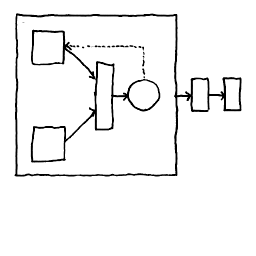
\includegraphics[width = 5cm]{../TikZ/drawings/expert-1.png}&
            \includegraphics[width = 5cm]{../TikZ/drawings/expert-1-parses/0.png}&
    
        \begin{minipage}{10cm}
        \begin{verbatim}
Solver timeout
        \end{verbatim}
\end{minipage}

    \end{tabular}        
            \\

            \begin{tabular}{lll}
    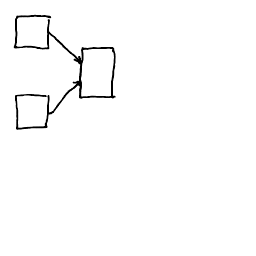
\includegraphics[width = 5cm]{../TikZ/drawings/expert-2.png}&
            \includegraphics[width = 5cm]{../TikZ/drawings/expert-2-parses/0.png}&
    
        \begin{minipage}{10cm}
        \begin{verbatim}
rectangle(4,2,6,5);
reflect(reflect(y = 7)){
line(2,6,4,4,
arrow = True,solid = True);
rectangle(0,0,2,2)
}
        \end{verbatim}
\end{minipage}

    \end{tabular}        
            \\

            \begin{tabular}{lll}
    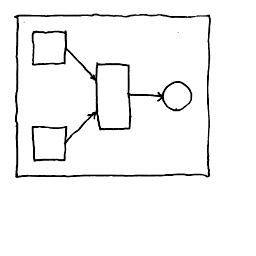
\includegraphics[width = 5cm]{../TikZ/drawings/expert-3.png}&
            \includegraphics[width = 5cm]{../TikZ/drawings/expert-3-parses/0.png}&
    
        \begin{minipage}{10cm}
        \begin{verbatim}
circle(10,5);
line(7,5,9,5,
arrow = True,solid = True);
rectangle(5,3,7,7);
rectangle(0,0,12,10);
reflect(reflect(y = 10)){
line(3,8,5,6,
arrow = True,solid = True);
rectangle(1,7,3,9)
}
        \end{verbatim}
\end{minipage}

    \end{tabular}        
            \\

            \begin{tabular}{lll}
    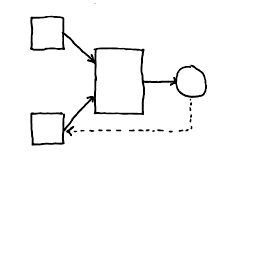
\includegraphics[width = 5cm]{../TikZ/drawings/expert-4.png}&
            \includegraphics[width = 5cm]{../TikZ/drawings/expert-4-parses/0.png}&
    
        \begin{minipage}{10cm}
        \begin{verbatim}
circle(10,4);
line(10,1,2,1,
arrow = True,solid = False);
line(10,1,10,3,
arrow = False,solid = False);
line(7,4,9,4,
arrow = True,solid = True);
reflect(reflect(y = 8)){
line(2,7,4,5,
arrow = True,solid = True);
rectangle(4,2,7,6);
rectangle(0,6,2,8)
}
        \end{verbatim}
\end{minipage}

    \end{tabular}        
            \\

            \begin{tabular}{lll}
    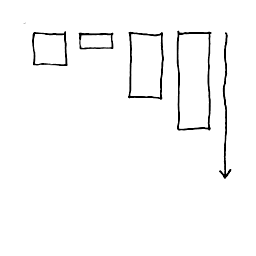
\includegraphics[width = 5cm]{../TikZ/drawings/expert-5.png}&
            \includegraphics[width = 5cm]{../TikZ/drawings/expert-5-parses/0.png}&
    
        \begin{minipage}{10cm}
        \begin{verbatim}
Solver timeout
        \end{verbatim}
\end{minipage}

    \end{tabular}        
            \\

            \begin{tabular}{lll}
    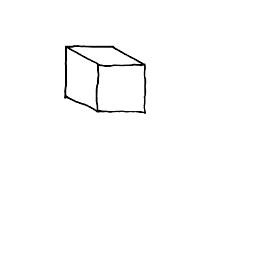
\includegraphics[width = 5cm]{../TikZ/drawings/expert-6.png}&
            \includegraphics[width = 5cm]{../TikZ/drawings/expert-6-parses/0.png}&
    
        \begin{minipage}{10cm}
        \begin{verbatim}
line(0,1,2,0,
arrow = False,solid = True);
for (i < 3){
if (i > 0){
line(3*i + -3,4,3*i + -1,3,
arrow = False,solid = True);
line(0,3*i + -2,3*i + -3,4,
arrow = False,solid = True)
}
rectangle(2,0,5,3)
}
        \end{verbatim}
\end{minipage}

    \end{tabular}        
            \\

            \begin{tabular}{lll}
    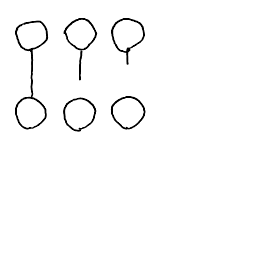
\includegraphics[width = 5cm]{../TikZ/drawings/expert-7.png}&
            \includegraphics[width = 5cm]{../TikZ/drawings/expert-7-parses/0.png}&
    
        \begin{minipage}{10cm}
        \begin{verbatim}
for (i < 3){
circle(-3*i + 7,1);
circle(-3*i + 7,6);
line(-3*i + 7,-1*i + 4,-3*i + 7,5,
arrow = False,solid = True)
}
        \end{verbatim}
\end{minipage}

    \end{tabular}        
            \\

            \begin{tabular}{lll}
    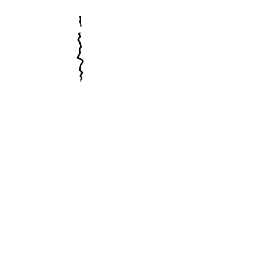
\includegraphics[width = 5cm]{../TikZ/drawings/expert-8.png}&
            \includegraphics[width = 5cm]{../TikZ/drawings/expert-8-parses/0.png}&
    
        \begin{minipage}{10cm}
        \begin{verbatim}
line(0,0,0,4,
arrow = False,solid = True)
        \end{verbatim}
\end{minipage}

    \end{tabular}        
            \\

            \begin{tabular}{lll}
    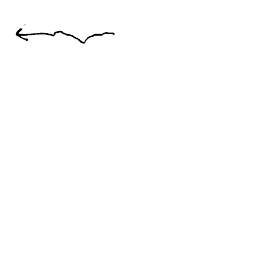
\includegraphics[width = 5cm]{../TikZ/drawings/expert-9.png}&
            \includegraphics[width = 5cm]{../TikZ/drawings/expert-9-parses/0.png}&
    
        \begin{minipage}{10cm}
        \begin{verbatim}
line(6,0,0,0,
arrow = True,solid = True)
        \end{verbatim}
\end{minipage}

    \end{tabular}        
            \\

            \begin{tabular}{lll}
    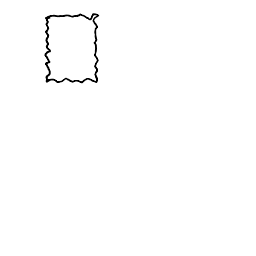
\includegraphics[width = 5cm]{../TikZ/drawings/expert-10.png}&
            \includegraphics[width = 5cm]{../TikZ/drawings/expert-10-parses/0.png}&
    
        \begin{minipage}{10cm}
        \begin{verbatim}
rectangle(0,0,3,4)
        \end{verbatim}
\end{minipage}

    \end{tabular}        
            \\

            \begin{tabular}{lll}
    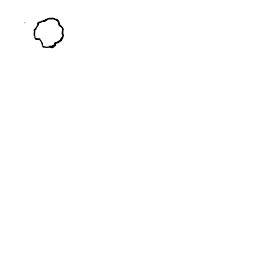
\includegraphics[width = 5cm]{../TikZ/drawings/expert-11.png}&
            \includegraphics[width = 5cm]{../TikZ/drawings/expert-11-parses/0.png}&
    
        \begin{minipage}{10cm}
        \begin{verbatim}
circle(1,1)
        \end{verbatim}
\end{minipage}

    \end{tabular}        
            \\

            \begin{tabular}{lll}
    \includegraphics[width = 5cm]{../TikZ/drawings/expert-12.png}&
            \includegraphics[width = 5cm]{../TikZ/drawings/expert-12-parses/0.png}&
    
        \begin{minipage}{10cm}
        \begin{verbatim}
line(2,6,5,6,
arrow = False,solid = True);
reflect(reflect(x = 7)){
circle(6,1);
line(2,1,5,1,
arrow = False,solid = True);
line(1,2,1,5,
arrow = False,solid = True);
rectangle(5,5,7,7)
}
        \end{verbatim}
\end{minipage}

    \end{tabular}        
            \\

            \begin{tabular}{lll}
    \includegraphics[width = 5cm]{../TikZ/drawings/expert-13.png}&
            \includegraphics[width = 5cm]{../TikZ/drawings/expert-13-parses/0.png}&
    
        \begin{minipage}{10cm}
        \begin{verbatim}
line(2,1,4,1,
arrow = True,solid = True);
line(3,2,1,2,
arrow = True,solid = True);
line(5,0,3,0,
arrow = True,solid = True);
line(0,3,2,3,
arrow = True,solid = True)
        \end{verbatim}
\end{minipage}

    \end{tabular}        
            \\

            \begin{tabular}{lll}
    \includegraphics[width = 5cm]{../TikZ/drawings/expert-14.png}&
            \includegraphics[width = 5cm]{../TikZ/drawings/expert-14-parses/0.png}&
    
        \begin{minipage}{10cm}
        \begin{verbatim}
for (i < 4){
if (i > 0){
rectangle(-2*i + 6,2*i + -2,-2*i + 7,2*i + -1)
}
rectangle(-2*i + 6,2*i,-2*i + 7,2*i + 1)
}
        \end{verbatim}
\end{minipage}

    \end{tabular}        
            \\

            \begin{tabular}{lll}
    \includegraphics[width = 5cm]{../TikZ/drawings/expert-15.png}&
            \includegraphics[width = 5cm]{../TikZ/drawings/expert-15-parses/0.png}&
    
        \begin{minipage}{10cm}
        \begin{verbatim}
line(0,3,2,3,
arrow = False,solid = False);
line(2,1,4,1,
arrow = False,solid = False);
line(1,2,3,2,
arrow = False,solid = True);
line(3,0,5,0,
arrow = False,solid = True)
        \end{verbatim}
\end{minipage}

    \end{tabular}        
            \\

            \begin{tabular}{lll}
    \includegraphics[width = 5cm]{../TikZ/drawings/expert-16.png}&
            \includegraphics[width = 5cm]{../TikZ/drawings/expert-16-parses/0.png}&
    
        \begin{minipage}{10cm}
        \begin{verbatim}
for (i < 4){
if (i > 0){
circle(-2*i + 7,3*i + -2);
line(-2*i + 9,3*i,-2*i + 10,3*i + -2,
arrow = False,solid = True);
line(-2*i + 8,3*i + -2,-2*i + 9,3*i,
arrow = False,solid = True)
}
circle(-2*i + 9,3*i + 1)
}
        \end{verbatim}
\end{minipage}

    \end{tabular}        
            \\

            \begin{tabular}{lll}
    \includegraphics[width = 5cm]{../TikZ/drawings/expert-17.png}&
            \includegraphics[width = 5cm]{../TikZ/drawings/expert-17-parses/0.png}&
    
        \begin{minipage}{10cm}
        \begin{verbatim}
for (i < 4){
if (i > 0){
line(2*i + 1,-3*i + 12,2*i,-3*i + 10,
arrow = True,solid = True);
line(2*i + 1,-3*i + 12,2*i + 2,-3*i + 10,
arrow = True,solid = True);
rectangle(2*i + -2,-3*i + 9,2*i,-3*i + 11)
}
rectangle(2*i + 2,-3*i + 9,2*i + 4,-3*i + 11)
}
        \end{verbatim}
\end{minipage}

    \end{tabular}        
            \\

            \begin{tabular}{lll}
    \includegraphics[width = 5cm]{../TikZ/drawings/expert-18.png}&
            \includegraphics[width = 5cm]{../TikZ/drawings/expert-18-parses/0.png}&
    
        \begin{minipage}{10cm}
        \begin{verbatim}
circle(5,1);
for (i < 3){
if (i > 0){
circle(7,2*i + -1);
circle(i + 2,2*i + 1)
}
circle(1,6)
}
        \end{verbatim}
\end{minipage}

    \end{tabular}        
            \\

            \begin{tabular}{lll}
    \includegraphics[width = 5cm]{../TikZ/drawings/expert-19.png}&
            \includegraphics[width = 5cm]{../TikZ/drawings/expert-19-parses/0.png}&
    
        \begin{minipage}{10cm}
        \begin{verbatim}
line(4,4,2,2,
arrow = True,solid = True);
rectangle(3,4,5,6);
rectangle(0,0,2,2)
        \end{verbatim}
\end{minipage}

    \end{tabular}        
            \\

            \begin{tabular}{lll}
    \includegraphics[width = 5cm]{../TikZ/drawings/expert-20.png}&
            \includegraphics[width = 5cm]{../TikZ/drawings/expert-20-parses/0.png}&
    
        \begin{minipage}{10cm}
        \begin{verbatim}
rectangle(0,4,2,6);
for (i < 3){
if (i > 0){
line(-4*i + 12,5,-4*i + 10,5,
arrow = True,solid = True);
for (j < i + 1){
circle(-4*j + 9,-4*i + 9)
}
}
line(-4*i + 9,4,-4*i + 9,2,
arrow = True,solid = True)
}
        \end{verbatim}
\end{minipage}

    \end{tabular}        
            \\

            \begin{tabular}{lll}
    \includegraphics[width = 5cm]{../TikZ/drawings/expert-21.png}&
            \includegraphics[width = 5cm]{../TikZ/drawings/expert-21-parses/0.png}&
    
        \begin{minipage}{10cm}
        \begin{verbatim}
Solver timeout
        \end{verbatim}
\end{minipage}

    \end{tabular}        
            \\

            \begin{tabular}{lll}
    \includegraphics[width = 5cm]{../TikZ/drawings/expert-22.png}&
            \includegraphics[width = 5cm]{../TikZ/drawings/expert-22-parses/0.png}&
    
        \begin{minipage}{10cm}
        \begin{verbatim}
for (i < 3){
line(-4*i + 9,4,-4*i + 9,2,
arrow = True,solid = True);
for (j < 2){
line(-4*j + 8,5,-4*j + 6,5,
arrow = True,solid = True);
rectangle(-4*i + 8,4*j,-4*i + 10,4*j + 2)
}
}
        \end{verbatim}
\end{minipage}

    \end{tabular}        
            \\

            \begin{tabular}{lll}
    \includegraphics[width = 5cm]{../TikZ/drawings/expert-23.png}&
            \includegraphics[width = 5cm]{../TikZ/drawings/expert-23-parses/0.png}&
    
        \begin{minipage}{10cm}
        \begin{verbatim}
for (i < 3){
if (i > 0){
line(-4*i + 12,1,-4*i + 10,1,
arrow = True,solid = True)
}
circle(-4*i + 9,1);
circle(-4*i + 9,5);
line(-4*i + 9,2,-4*i + 9,4,
arrow = True,solid = True)
}
        \end{verbatim}
\end{minipage}

    \end{tabular}        
            \\

            \begin{tabular}{lll}
    \includegraphics[width = 5cm]{../TikZ/drawings/expert-24.png}&
            \includegraphics[width = 5cm]{../TikZ/drawings/expert-24-parses/0.png}&
    
        \begin{minipage}{10cm}
        \begin{verbatim}
reflect(reflect(x = 6)){
for (i < 3){
if (i > 0){
line(-2*i + 7,-4*i + 11,-2*i + 7,-4*i + 10,
arrow = True,solid = True);
rectangle(0,-4*i + 11,6,-3*i + 12)
}
rectangle(2,0,4,2)
}
}
        \end{verbatim}
\end{minipage}

    \end{tabular}        
            \\

            \begin{tabular}{lll}
    \includegraphics[width = 5cm]{../TikZ/drawings/expert-25.png}&
            \includegraphics[width = 5cm]{../TikZ/drawings/expert-25-parses/0.png}&
    
        \begin{minipage}{10cm}
        \begin{verbatim}
for (i < 3){
if (i > 0){
line(3*i,1,3*i + -1,1,
arrow = True,solid = True)
}
rectangle(3*i,0,3*i + 2,2)
}
        \end{verbatim}
\end{minipage}

    \end{tabular}        
            \\

            \begin{tabular}{lll}
    \includegraphics[width = 5cm]{../TikZ/drawings/expert-26.png}&
            \includegraphics[width = 5cm]{../TikZ/drawings/expert-26-parses/0.png}&
    
        \begin{minipage}{10cm}
        \begin{verbatim}
line(1,3,1,4,
arrow = False,solid = True);
for (i < 3){
if (i > 0){
line(1,-5*i + 13,1,-4*i + 10,
arrow = True,solid = True)
}
circle(1,-4*i + 9)
}
        \end{verbatim}
\end{minipage}

    \end{tabular}        
            \\

            \begin{tabular}{lll}
    \includegraphics[width = 5cm]{../TikZ/drawings/expert-27.png}&
            \includegraphics[width = 5cm]{../TikZ/drawings/expert-27-parses/0.png}&
    
        \begin{minipage}{10cm}
        \begin{verbatim}
reflect(reflect(x = 2)){
line(0,1,1,2,
arrow = False,solid = True);
line(1,0,2,1,
arrow = False,solid = True)
}
        \end{verbatim}
\end{minipage}

    \end{tabular}        
            \\

            \begin{tabular}{lll}
    \includegraphics[width = 5cm]{../TikZ/drawings/expert-28.png}&
            \includegraphics[width = 5cm]{../TikZ/drawings/expert-28-parses/0.png}&
    
        \begin{minipage}{10cm}
        \begin{verbatim}
line(0,0,0,2,
arrow = False,solid = True);
line(0,2,2,2,
arrow = False,solid = True)
        \end{verbatim}
\end{minipage}

    \end{tabular}        
            \\

            \begin{tabular}{lll}
    \includegraphics[width = 5cm]{../TikZ/drawings/expert-29.png}&
            \includegraphics[width = 5cm]{../TikZ/drawings/expert-29-parses/0.png}&
    
        \begin{minipage}{10cm}
        \begin{verbatim}
for (i < 3){
line(i,-1*i + 6,2*i + 2,-1*i + 6,
arrow = False,solid = True);
line(i,-2*i + 4,i,-1*i + 6,
arrow = False,solid = True)
}
        \end{verbatim}
\end{minipage}

    \end{tabular}        
            \\

            \begin{tabular}{lll}
    \includegraphics[width = 5cm]{../TikZ/drawings/expert-30.png}&
            \includegraphics[width = 5cm]{../TikZ/drawings/expert-30-parses/0.png}&
    
        \begin{minipage}{10cm}
        \begin{verbatim}
for (i < 3){
if (i > 0){
circle(1,-3*i + 7);
circle(5,-2*i + 6);
rectangle(0,-3*i + 6,2,-3*i + 8)
}
rectangle(4,1,6,5)
}
        \end{verbatim}
\end{minipage}

    \end{tabular}        
            \\

            \begin{tabular}{lll}
    \includegraphics[width = 5cm]{../TikZ/drawings/expert-31.png}&
            \includegraphics[width = 5cm]{../TikZ/drawings/expert-31-parses/0.png}&
    
        \begin{minipage}{10cm}
        \begin{verbatim}
for (i < 3){
rectangle(3*i,-2*i + 4,3*i + 2,6);
for (j < i + 1){
circle(3*i + 1,-2*j + 5)
}
}
        \end{verbatim}
\end{minipage}

    \end{tabular}        
            \\

            \begin{tabular}{lll}
    \includegraphics[width = 5cm]{../TikZ/drawings/expert-32.png}&
            \includegraphics[width = 5cm]{../TikZ/drawings/expert-32-parses/0.png}&
    
        \begin{minipage}{10cm}
        \begin{verbatim}
circle(5,5);
line(2,5,4,5,
arrow = False,solid = True);
rectangle(0,0,5,3);
rectangle(0,4,2,6)
        \end{verbatim}
\end{minipage}

    \end{tabular}        
            \\

            \begin{tabular}{lll}
    \includegraphics[width = 5cm]{../TikZ/drawings/expert-33.png}&
            \includegraphics[width = 5cm]{../TikZ/drawings/expert-33-parses/0.png}&
    
        \begin{minipage}{10cm}
        \begin{verbatim}
line(0,0,6,0,
arrow = False,solid = False);
reflect(reflect(x = 6)){
line(6,0,6,3,
arrow = False,solid = True);
line(0,3,6,3,
arrow = False,solid = False)
}
        \end{verbatim}
\end{minipage}

    \end{tabular}        
            \\

            \begin{tabular}{lll}
    \includegraphics[width = 5cm]{../TikZ/drawings/expert-34.png}&
            \includegraphics[width = 5cm]{../TikZ/drawings/expert-34-parses/0.png}&
    
        \begin{minipage}{10cm}
        \begin{verbatim}
Solver timeout
        \end{verbatim}
\end{minipage}

    \end{tabular}        
            \\

            \begin{tabular}{lll}
    \includegraphics[width = 5cm]{../TikZ/drawings/expert-35.png}&
            \includegraphics[width = 5cm]{../TikZ/drawings/expert-35-parses/0.png}&
    
        \begin{minipage}{10cm}
        \begin{verbatim}
for (i < 3){
if (i > 0){
circle(-5*i + 11,1);
line(-1*i + 3,-1*i + 7,-5*i + 11,2,
arrow = True,solid = True)
}
circle(1,6)
}
        \end{verbatim}
\end{minipage}

    \end{tabular}        
            \\

            \begin{tabular}{lll}
    \includegraphics[width = 5cm]{../TikZ/drawings/expert-36.png}&
            \includegraphics[width = 5cm]{../TikZ/drawings/expert-36-parses/0.png}&
    
        \begin{minipage}{10cm}
        \begin{verbatim}
Solver timeout
        \end{verbatim}
\end{minipage}

    \end{tabular}        
            \\

            \begin{tabular}{lll}
    \includegraphics[width = 5cm]{../TikZ/drawings/expert-37.png}&
            \includegraphics[width = 5cm]{../TikZ/drawings/expert-37-parses/0.png}&
    
        \begin{minipage}{10cm}
        \begin{verbatim}
for (i < 3){
if (i > 0){
line(4*i + -3,-5*i + 12,2*i + 1,5,
arrow = False,solid = True);
rectangle(4*i + -4,-5*i + 10,6,-7*i + 16)
}
circle(1,8)
}
        \end{verbatim}
\end{minipage}

    \end{tabular}        
            \\

            \begin{tabular}{lll}
    \includegraphics[width = 5cm]{../TikZ/drawings/expert-38.png}&
            \includegraphics[width = 5cm]{../TikZ/drawings/expert-38-parses/0.png}&
    
        \begin{minipage}{10cm}
        \begin{verbatim}
Solver timeout
        \end{verbatim}
\end{minipage}

    \end{tabular}        
            \\

            \begin{tabular}{lll}
    \includegraphics[width = 5cm]{../TikZ/drawings/expert-39.png}&
            \includegraphics[width = 5cm]{../TikZ/drawings/expert-39-parses/0.png}&
    
        \begin{minipage}{10cm}
        \begin{verbatim}
Solver timeout
        \end{verbatim}
\end{minipage}

    \end{tabular}        
            \\

            \begin{tabular}{lll}
    \includegraphics[width = 5cm]{../TikZ/drawings/expert-40.png}&
            \includegraphics[width = 5cm]{../TikZ/drawings/expert-40-parses/0.png}&
    
        \begin{minipage}{10cm}
        \begin{verbatim}
for (i < 3){
circle(-3*i + 7,1)
}
        \end{verbatim}
\end{minipage}

    \end{tabular}        
            \\

            \begin{tabular}{lll}
    \includegraphics[width = 5cm]{../TikZ/drawings/expert-41.png}&
            \includegraphics[width = 5cm]{../TikZ/drawings/expert-41-parses/0.png}&
    
        \begin{minipage}{10cm}
        \begin{verbatim}
for (i < 3){
rectangle(-2*i + 4,0,-2*i + 5,6)
}
        \end{verbatim}
\end{minipage}

    \end{tabular}        
            \\

            \begin{tabular}{lll}
    \includegraphics[width = 5cm]{../TikZ/drawings/expert-42.png}&
            \includegraphics[width = 5cm]{../TikZ/drawings/expert-42-parses/0.png}&
    
        \begin{minipage}{10cm}
        \begin{verbatim}
line(4,0,4,1,
arrow = False,solid = False);
line(0,0,0,5,
arrow = False,solid = False);
line(4,1,4,5,
arrow = False,solid = False)
        \end{verbatim}
\end{minipage}

    \end{tabular}        
            \\

            \begin{tabular}{lll}
    \includegraphics[width = 5cm]{../TikZ/drawings/expert-43.png}&
            \includegraphics[width = 5cm]{../TikZ/drawings/expert-43-parses/0.png}&
    
        \begin{minipage}{10cm}
        \begin{verbatim}
line(4,0,4,5,
arrow = False,solid = True);
line(0,0,0,5,
arrow = False,solid = True)
        \end{verbatim}
\end{minipage}

    \end{tabular}        
            \\

            \begin{tabular}{lll}
    \includegraphics[width = 5cm]{../TikZ/drawings/expert-44.png}&
            \includegraphics[width = 5cm]{../TikZ/drawings/expert-44-parses/0.png}&
    
        \begin{minipage}{10cm}
        \begin{verbatim}
reflect(reflect(x = 12)){
circle(4,1);
line(9,1,10,1,
arrow = False,solid = True);
rectangle(0,0,2,2)
}
        \end{verbatim}
\end{minipage}

    \end{tabular}        
            \\

            \begin{tabular}{lll}
    \includegraphics[width = 5cm]{../TikZ/drawings/expert-45.png}&
            \includegraphics[width = 5cm]{../TikZ/drawings/expert-45-parses/0.png}&
    
        \begin{minipage}{10cm}
        \begin{verbatim}
rectangle(0,4,4,8);
reflect(reflect(y = 12)){
circle(7,6);
line(2,2,2,4,
arrow = True,solid = True);
line(4,6,6,6,
arrow = True,solid = True);
rectangle(1,10,3,12)
}
        \end{verbatim}
\end{minipage}

    \end{tabular}        
            \\

            \begin{tabular}{lll}
    \includegraphics[width = 5cm]{../TikZ/drawings/expert-46.png}&
            \includegraphics[width = 5cm]{../TikZ/drawings/expert-46-parses/0.png}&
    
        \begin{minipage}{10cm}
        \begin{verbatim}
reflect(reflect(y = 9)){
line(3,8,6,8,
arrow = False,solid = True);
reflect(reflect(x = 9)){
circle(1,8);
line(1,3,1,6,
arrow = False,solid = True)
}
}
        \end{verbatim}
\end{minipage}

    \end{tabular}        
            \\

            \begin{tabular}{lll}
    \includegraphics[width = 5cm]{../TikZ/drawings/expert-47.png}&
            \includegraphics[width = 5cm]{../TikZ/drawings/expert-47-parses/0.png}&
    
        \begin{minipage}{10cm}
        \begin{verbatim}
reflect(reflect(y = 11)){
rectangle(4,9,7,10);
reflect(reflect(x = 11)){
rectangle(1,4,2,7);
rectangle(8,8,11,11)
}
}
        \end{verbatim}
\end{minipage}

    \end{tabular}        
            \\

            \begin{tabular}{lll}
    \includegraphics[width = 5cm]{../TikZ/drawings/expert-48.png}&
            \includegraphics[width = 5cm]{../TikZ/drawings/expert-48-parses/0.png}&
    
        \begin{minipage}{10cm}
        \begin{verbatim}
for (i < 4){
line(i,-1*i + 5,i + 2,-1*i + 5,
arrow = False,solid = True);
line(i + 2,-1*i + 3,i + 4,-1*i + 3,
arrow = False,solid = True)
}
        \end{verbatim}
\end{minipage}

    \end{tabular}        
            \\

            \begin{tabular}{lll}
    \includegraphics[width = 5cm]{../TikZ/drawings/expert-49.png}&
            \includegraphics[width = 5cm]{../TikZ/drawings/expert-49-parses/0.png}&
    
        \begin{minipage}{10cm}
        \begin{verbatim}
for (i < 3){
if (i > 0){
rectangle(3*i + 1,-1*i + 2,3*i + 3,2);
rectangle(0,7*i + -7,3,7*i + -4)
}
rectangle(1,4,2,6)
}
        \end{verbatim}
\end{minipage}

    \end{tabular}        
            \\

            \begin{tabular}{lll}
    \includegraphics[width = 5cm]{../TikZ/drawings/expert-50.png}&
            \includegraphics[width = 5cm]{../TikZ/drawings/expert-50-parses/0.png}&
    
        \begin{minipage}{10cm}
        \begin{verbatim}
Solver timeout
        \end{verbatim}
\end{minipage}

    \end{tabular}        
            \\

            \begin{tabular}{lll}
    \includegraphics[width = 5cm]{../TikZ/drawings/expert-51.png}&
            \includegraphics[width = 5cm]{../TikZ/drawings/expert-51-parses/0.png}&
    
        \begin{minipage}{10cm}
        \begin{verbatim}
for (i < 3){
rectangle(-2*i + 4,-2*i + 4,-2*i + 7,-2*i + 5)
}
        \end{verbatim}
\end{minipage}

    \end{tabular}        
            \\

            \begin{tabular}{lll}
    \includegraphics[width = 5cm]{../TikZ/drawings/expert-52.png}&
            \includegraphics[width = 5cm]{../TikZ/drawings/expert-52-parses/0.png}&
    
        \begin{minipage}{10cm}
        \begin{verbatim}
circle(4,10);
for (i < 3){
circle(-3*i + 7,5);
circle(-3*i + 7,1);
line(-3*i + 7,4,-3*i + 7,2,
arrow = True,solid = True);
line(4,9,-3*i + 7,6,
arrow = True,solid = True)
}
        \end{verbatim}
\end{minipage}

    \end{tabular}        
            \\

            \begin{tabular}{lll}
    \includegraphics[width = 5cm]{../TikZ/drawings/expert-53.png}&
            \includegraphics[width = 5cm]{../TikZ/drawings/expert-53-parses/0.png}&
    
        \begin{minipage}{10cm}
        \begin{verbatim}
line(2,8,2,6,
arrow = True,solid = True);
line(6,8,6,4,
arrow = True,solid = True);
line(4,8,4,0,
arrow = True,solid = True);
line(0,8,8,8,
arrow = False,solid = True)
        \end{verbatim}
\end{minipage}

    \end{tabular}        
            \\

            \begin{tabular}{lll}
    \includegraphics[width = 5cm]{../TikZ/drawings/expert-54.png}&
            \includegraphics[width = 5cm]{../TikZ/drawings/expert-54-parses/0.png}&
    
        \begin{minipage}{10cm}
        \begin{verbatim}
line(2,3,2,5,
arrow = False,solid = True);
rectangle(1,1,3,3);
rectangle(1,5,3,7);
rectangle(0,0,4,8)
        \end{verbatim}
\end{minipage}

    \end{tabular}        
            \\

            \begin{tabular}{lll}
    \includegraphics[width = 5cm]{../TikZ/drawings/expert-55.png}&
            \includegraphics[width = 5cm]{../TikZ/drawings/expert-55-parses/0.png}&
    
        \begin{minipage}{10cm}
        \begin{verbatim}
circle(1,5);
line(1,4,1,2,
arrow = True,solid = True);
rectangle(0,0,2,2)
        \end{verbatim}
\end{minipage}

    \end{tabular}        
            \\

            \begin{tabular}{lll}
    \includegraphics[width = 5cm]{../TikZ/drawings/expert-56.png}&
            \includegraphics[width = 5cm]{../TikZ/drawings/expert-56-parses/0.png}&
    
        \begin{minipage}{10cm}
        \begin{verbatim}
Solver timeout
        \end{verbatim}
\end{minipage}

    \end{tabular}        
            \\

            \begin{tabular}{lll}
    \includegraphics[width = 5cm]{../TikZ/drawings/expert-57.png}&
            \includegraphics[width = 5cm]{../TikZ/drawings/expert-57-parses/0.png}&
    
        \begin{minipage}{10cm}
        \begin{verbatim}
for (i < 3){
for (j < 3){
circle(-4*j + 9,-3*i + 7)
}
}
        \end{verbatim}
\end{minipage}

    \end{tabular}        
            \\

            \begin{tabular}{lll}
    \includegraphics[width = 5cm]{../TikZ/drawings/expert-58.png}&
            \includegraphics[width = 5cm]{../TikZ/drawings/expert-58-parses/0.png}&
    
        \begin{minipage}{10cm}
        \begin{verbatim}
for (i < 3){
if (i > 0){
line(8,0,8*i + -8,7*i + -7,
arrow = True,solid = True)
}
rectangle(2*i + 2,0,2*i + 3,i + 3)
}
        \end{verbatim}
\end{minipage}

    \end{tabular}        
            \\

            \begin{tabular}{lll}
    \includegraphics[width = 5cm]{../TikZ/drawings/expert-59.png}&
            \includegraphics[width = 5cm]{../TikZ/drawings/expert-59-parses/0.png}&
    
        \begin{minipage}{10cm}
        \begin{verbatim}
line(4,0,0,0,
arrow = False,solid = False)
        \end{verbatim}
\end{minipage}

    \end{tabular}        
            \\

            \begin{tabular}{lll}
    \includegraphics[width = 5cm]{../TikZ/drawings/expert-60.png}&
            \includegraphics[width = 5cm]{../TikZ/drawings/expert-60-parses/0.png}&
    
        \begin{minipage}{10cm}
        \begin{verbatim}
Solver timeout
        \end{verbatim}
\end{minipage}

    \end{tabular}        
            \\

            \begin{tabular}{lll}
    \includegraphics[width = 5cm]{../TikZ/drawings/expert-61.png}&
            \includegraphics[width = 5cm]{../TikZ/drawings/expert-61-parses/0.png}&
    
        \begin{minipage}{10cm}
        \begin{verbatim}
circle(2,1);
circle(6,1);
line(5,1,3,1,
arrow = True,solid = True);
rectangle(0,0,7,2)
        \end{verbatim}
\end{minipage}

    \end{tabular}        
            \\

            \begin{tabular}{lll}
    \includegraphics[width = 5cm]{../TikZ/drawings/expert-62.png}&
            \includegraphics[width = 5cm]{../TikZ/drawings/expert-62-parses/0.png}&
    
        \begin{minipage}{10cm}
        \begin{verbatim}
rectangle(5,0,8,3);
rectangle(2,1,4,3);
rectangle(0,2,1,3)
        \end{verbatim}
\end{minipage}

    \end{tabular}        
            \\

            \begin{tabular}{lll}
    \includegraphics[width = 5cm]{../TikZ/drawings/expert-63.png}&
            \includegraphics[width = 5cm]{../TikZ/drawings/expert-63-parses/0.png}&
    
        \begin{minipage}{10cm}
        \begin{verbatim}
for (i < 3){
rectangle(-1*i + 2,-1*i + 2,i + 3,i + 3)
}
        \end{verbatim}
\end{minipage}

    \end{tabular}        
            \\

            \begin{tabular}{lll}
    \includegraphics[width = 5cm]{../TikZ/drawings/expert-64.png}&
            \includegraphics[width = 5cm]{../TikZ/drawings/expert-64-parses/0.png}&
    
        \begin{minipage}{10cm}
        \begin{verbatim}
reflect(reflect(x = 6)){
line(5,2,5,4,
arrow = False,solid = True);
reflect(reflect(y = 6)){
line(2,1,4,1,
arrow = False,solid = True);
rectangle(4,4,6,6)
}
}
        \end{verbatim}
\end{minipage}

    \end{tabular}        
            \\

            \begin{tabular}{lll}
    \includegraphics[width = 5cm]{../TikZ/drawings/expert-65.png}&
            \includegraphics[width = 5cm]{../TikZ/drawings/expert-65-parses/0.png}&
    
        \begin{minipage}{10cm}
        \begin{verbatim}
reflect(reflect(y = 6)){
line(2,5,4,5,
arrow = False,solid = True);
reflect(reflect(x = 6)){
circle(5,5);
line(1,2,1,4,
arrow = False,solid = True)
}
}
        \end{verbatim}
\end{minipage}

    \end{tabular}        
            \\

            \begin{tabular}{lll}
    \includegraphics[width = 5cm]{../TikZ/drawings/expert-66.png}&
            \includegraphics[width = 5cm]{../TikZ/drawings/expert-66-parses/0.png}&
    
        \begin{minipage}{10cm}
        \begin{verbatim}
for (i < 3){
line(i,-1*i + 2,-1*i + 7,-1*i + 2,
arrow = False,solid = True)
}
        \end{verbatim}
\end{minipage}

    \end{tabular}        
            \\

            \begin{tabular}{lll}
    \includegraphics[width = 5cm]{../TikZ/drawings/expert-67.png}&
            \includegraphics[width = 5cm]{../TikZ/drawings/expert-67-parses/0.png}&
    
        \begin{minipage}{10cm}
        \begin{verbatim}
line(1,4,5,0,
arrow = False,solid = True);
line(1,5,5,1,
arrow = False,solid = True);
rectangle(5,0,6,1);
rectangle(0,4,1,5)
        \end{verbatim}
\end{minipage}

    \end{tabular}        
            \\

            \begin{tabular}{lll}
    \includegraphics[width = 5cm]{../TikZ/drawings/expert-68.png}&
            \includegraphics[width = 5cm]{../TikZ/drawings/expert-68-parses/0.png}&
    
        \begin{minipage}{10cm}
        \begin{verbatim}
for (i < 3){
circle(4*i + 1,1);
rectangle(4*i,0,4*i + 2,2)
}
        \end{verbatim}
\end{minipage}

    \end{tabular}        
            \\

            \begin{tabular}{lll}
    \includegraphics[width = 5cm]{../TikZ/drawings/expert-69.png}&
            \includegraphics[width = 5cm]{../TikZ/drawings/expert-69-parses/0.png}&
    
        \begin{minipage}{10cm}
        \begin{verbatim}
reflect(reflect(x = 5)){
circle(1,1);
line(4,4,4,2,
arrow = True,solid = True);
rectangle(0,4,5,6)
}
        \end{verbatim}
\end{minipage}

    \end{tabular}        
            \\

            \begin{tabular}{lll}
    \includegraphics[width = 5cm]{../TikZ/drawings/expert-70.png}&
            \includegraphics[width = 5cm]{../TikZ/drawings/expert-70-parses/0.png}&
    
        \begin{minipage}{10cm}
        \begin{verbatim}
Solver timeout
        \end{verbatim}
\end{minipage}

    \end{tabular}        
            \\

            \begin{tabular}{lll}
    \includegraphics[width = 5cm]{../TikZ/drawings/expert-71.png}&
            Sampled no finished traces.&
    
        \begin{minipage}{10cm}
        \begin{verbatim}
Solver timeout
        \end{verbatim}
\end{minipage}

    \end{tabular}        
            \\

            \begin{tabular}{lll}
    \includegraphics[width = 5cm]{../TikZ/drawings/expert-72.png}&
            \includegraphics[width = 5cm]{../TikZ/drawings/expert-72-parses/0.png}&
    
        \begin{minipage}{10cm}
        \begin{verbatim}
reflect(reflect(y = 8)){
for (i < 3){
if (i > 0){
rectangle(3*i + -1,2,3*i,3)
}
circle(3*i + 1,3*i + 1)
}
}
        \end{verbatim}
\end{minipage}

    \end{tabular}        
            \\

            \begin{tabular}{lll}
    \includegraphics[width = 5cm]{../TikZ/drawings/expert-73.png}&
            Sampled no finished traces.&
    
        \begin{minipage}{10cm}
        \begin{verbatim}
Solver timeout
        \end{verbatim}
\end{minipage}

    \end{tabular}        
            \\

            \begin{tabular}{lll}
    \includegraphics[width = 5cm]{../TikZ/drawings/expert-74.png}&
            \includegraphics[width = 5cm]{../TikZ/drawings/expert-74-parses/0.png}&
    
        \begin{minipage}{10cm}
        \begin{verbatim}
for (i < 3){
if (i > 0){
rectangle(-2*i + 4,-2*i + 4,2*i + 2,2*i + 2)
}
for (j < 3){
circle(-2*i + 5,2*j + 1)
}
}
        \end{verbatim}
\end{minipage}

    \end{tabular}        
            \\

            \begin{tabular}{lll}
    \includegraphics[width = 5cm]{../TikZ/drawings/expert-75.png}&
            \includegraphics[width = 5cm]{../TikZ/drawings/expert-75-parses/0.png}&
    
        \begin{minipage}{10cm}
        \begin{verbatim}
for (i < 4){
line(-4*i + 13,4,-4*i + 13,2,
arrow = True,solid = True);
for (j < 3){
if (j > 0){
circle(-4*i + 13,4*j + -3)
}
line(-4*j + 10,5,-4*j + 12,5,
arrow = True,solid = True)
}
}
        \end{verbatim}
\end{minipage}

    \end{tabular}        
            \\

            \begin{tabular}{lll}
    \includegraphics[width = 5cm]{../TikZ/drawings/expert-76.png}&
            \includegraphics[width = 5cm]{../TikZ/drawings/expert-76-parses/0.png}&
    
        \begin{minipage}{10cm}
        \begin{verbatim}
circle(4,1);
reflect(reflect(x = 8)){
circle(1,8);
line(4,5,8,2,
arrow = False,solid = True);
line(4,5,4,10,
arrow = False,solid = True)
}
        \end{verbatim}
\end{minipage}

    \end{tabular}        
            \\

            \begin{tabular}{lll}
    \includegraphics[width = 5cm]{../TikZ/drawings/expert-77.png}&
            \includegraphics[width = 5cm]{../TikZ/drawings/expert-77-parses/0.png}&
    
        \begin{minipage}{10cm}
        \begin{verbatim}
Solver timeout
        \end{verbatim}
\end{minipage}

    \end{tabular}        
            \\

            \begin{tabular}{lll}
    \includegraphics[width = 5cm]{../TikZ/drawings/expert-78.png}&
            \includegraphics[width = 5cm]{../TikZ/drawings/expert-78-parses/0.png}&
    
        \begin{minipage}{10cm}
        \begin{verbatim}
line(0,6,12,6,
arrow = False,solid = True);
line(6,6,6,5,
arrow = True,solid = True);
line(8,3,7,4,
arrow = True,solid = True);
line(3,2,5,4,
arrow = True,solid = True);
reflect(reflect(x = 12)){
line(4,0,12,8,
arrow = False,solid = True)
}
        \end{verbatim}
\end{minipage}

    \end{tabular}        
            \\

            \begin{tabular}{lll}
    \includegraphics[width = 5cm]{../TikZ/drawings/expert-79.png}&
            \includegraphics[width = 5cm]{../TikZ/drawings/expert-79-parses/0.png}&
    
        \begin{minipage}{10cm}
        \begin{verbatim}
Solver timeout
        \end{verbatim}
\end{minipage}

    \end{tabular}        
            \\

            \begin{tabular}{lll}
    \includegraphics[width = 5cm]{../TikZ/drawings/expert-80.png}&
            \includegraphics[width = 5cm]{../TikZ/drawings/expert-80-parses/0.png}&
    
        \begin{minipage}{10cm}
        \begin{verbatim}
Solver timeout
        \end{verbatim}
\end{minipage}

    \end{tabular}        
            \\

            \begin{tabular}{lll}
    \includegraphics[width = 5cm]{../TikZ/drawings/expert-81.png}&
            \includegraphics[width = 5cm]{../TikZ/drawings/expert-81-parses/0.png}&
    
        \begin{minipage}{10cm}
        \begin{verbatim}
circle(1,1);
circle(4,1);
rectangle(9,0,11,2);
rectangle(6,0,8,2)
        \end{verbatim}
\end{minipage}

    \end{tabular}        
            \\

            \begin{tabular}{lll}
    \includegraphics[width = 5cm]{../TikZ/drawings/expert-82.png}&
            \includegraphics[width = 5cm]{../TikZ/drawings/expert-82-parses/0.png}&
    
        \begin{minipage}{10cm}
        \begin{verbatim}
Solver timeout
        \end{verbatim}
\end{minipage}

    \end{tabular}        
            \\

            \begin{tabular}{lll}
    \includegraphics[width = 5cm]{../TikZ/drawings/expert-83.png}&
            \includegraphics[width = 5cm]{../TikZ/drawings/expert-83-parses/0.png}&
    
        \begin{minipage}{10cm}
        \begin{verbatim}
Solver timeout
        \end{verbatim}
\end{minipage}

    \end{tabular}        
            \\

            \begin{tabular}{lll}
    \includegraphics[width = 5cm]{../TikZ/drawings/expert-84.png}&
            \includegraphics[width = 5cm]{../TikZ/drawings/expert-84-parses/0.png}&
    
        \begin{minipage}{10cm}
        \begin{verbatim}
Solver timeout
        \end{verbatim}
\end{minipage}

    \end{tabular}        
            \\

            \begin{tabular}{lll}
    \includegraphics[width = 5cm]{../TikZ/drawings/expert-85.png}&
            \includegraphics[width = 5cm]{../TikZ/drawings/expert-85-parses/0.png}&
    
        \begin{minipage}{10cm}
        \begin{verbatim}
for (i < 4){
if (i > 0){
line(1,-3*i + 12,1,-3*i + 11,
arrow = True,solid = True)
}
circle(1,-3*i + 10)
}
        \end{verbatim}
\end{minipage}

    \end{tabular}        
            \\

            \begin{tabular}{lll}
    \includegraphics[width = 5cm]{../TikZ/drawings/expert-86.png}&
            \includegraphics[width = 5cm]{../TikZ/drawings/expert-86-parses/0.png}&
    
        \begin{minipage}{10cm}
        \begin{verbatim}
Solver timeout
        \end{verbatim}
\end{minipage}

    \end{tabular}        
            \\

            \begin{tabular}{lll}
    \includegraphics[width = 5cm]{../TikZ/drawings/expert-87.png}&
            \includegraphics[width = 5cm]{../TikZ/drawings/expert-87-parses/0.png}&
    
        \begin{minipage}{10cm}
        \begin{verbatim}
reflect(reflect(x = 8)){
rectangle(0,5,3,8);
rectangle(0,2,2,4);
rectangle(0,0,1,1)
}
        \end{verbatim}
\end{minipage}

    \end{tabular}        
            \\

            \begin{tabular}{lll}
    \includegraphics[width = 5cm]{../TikZ/drawings/expert-88.png}&
            \includegraphics[width = 5cm]{../TikZ/drawings/expert-88-parses/0.png}&
    
        \begin{minipage}{10cm}
        \begin{verbatim}
for (i < 3){
rectangle(-2*i + 4,-1*i + 2,i + 6,2*i + 3)
}
        \end{verbatim}
\end{minipage}

    \end{tabular}        
            \\

            \begin{tabular}{lll}
    \includegraphics[width = 5cm]{../TikZ/drawings/expert-89.png}&
            \includegraphics[width = 5cm]{../TikZ/drawings/expert-89-parses/0.png}&
    
        \begin{minipage}{10cm}
        \begin{verbatim}
Solver timeout
        \end{verbatim}
\end{minipage}

    \end{tabular}        
            \\

            \begin{tabular}{lll}
    \includegraphics[width = 5cm]{../TikZ/drawings/expert-90.png}&
            \includegraphics[width = 5cm]{../TikZ/drawings/expert-90-parses/0.png}&
    
        \begin{minipage}{10cm}
        \begin{verbatim}
line(6,6,6,3,
arrow = True,solid = True);
for (i < 3){
if (i > 0){
circle(-5*i + 16,7);
circle(-5*i + 11,5*i + -3);
line(-5*i + 15,7,-5*i + 12,7,
arrow = True,solid = True)
}
rectangle(4,0,8,9)
}
        \end{verbatim}
\end{minipage}

    \end{tabular}        
            \\

            \begin{tabular}{lll}
    \includegraphics[width = 5cm]{../TikZ/drawings/expert-91.png}&
            \includegraphics[width = 5cm]{../TikZ/drawings/expert-91-parses/0.png}&
    
        \begin{minipage}{10cm}
        \begin{verbatim}
reflect(reflect(x = 5)){
reflect(reflect(y = 5)){
line(5,3,5,5,
arrow = False,solid = True);
line(3,5,5,5,
arrow = False,solid = True)
}
}
        \end{verbatim}
\end{minipage}

    \end{tabular}        
            \\

            \begin{tabular}{lll}
    \includegraphics[width = 5cm]{../TikZ/drawings/expert-92.png}&
            \includegraphics[width = 5cm]{../TikZ/drawings/expert-92-parses/0.png}&
    
        \begin{minipage}{10cm}
        \begin{verbatim}
reflect(reflect(x = 14)){
for (i < 3){
circle(9,-4*i + 9);
line(10,-4*i + 9,12,-4*i + 9,
arrow = False,solid = True);
rectangle(0,-4*i + 8,2,-4*i + 10)
}
}
        \end{verbatim}
\end{minipage}

    \end{tabular}        
            \\

            \begin{tabular}{lll}
    \includegraphics[width = 5cm]{../TikZ/drawings/expert-93.png}&
            \includegraphics[width = 5cm]{../TikZ/drawings/expert-93-parses/0.png}&
    
        \begin{minipage}{10cm}
        \begin{verbatim}
reflect(reflect(x = 10)){
for (i < 3){
if (i > 0){
line(4*i + -3,4*i + -2,4*i + 1,4*i,
arrow = True,solid = True)
}
circle(4*i + 1,4*i + 1)
}
}
        \end{verbatim}
\end{minipage}

    \end{tabular}        
            \\

            \begin{tabular}{lll}
    \includegraphics[width = 5cm]{../TikZ/drawings/expert-94.png}&
            Sampled no finished traces.&
    
        \begin{minipage}{10cm}
        \begin{verbatim}
line(0,2,12,2,
arrow = False,solid = True);
line(6,2,6,3,
arrow = True,solid = True);
reflect(reflect(x = 12)){
line(0,0,9,9,
arrow = False,solid = True);
line(10,7,7,4,
arrow = True,solid = True)
}
        \end{verbatim}
\end{minipage}

    \end{tabular}        
            \\

            \begin{tabular}{lll}
    \includegraphics[width = 5cm]{../TikZ/drawings/expert-95.png}&
            \includegraphics[width = 5cm]{../TikZ/drawings/expert-95-parses/0.png}&
    
        \begin{minipage}{10cm}
        \begin{verbatim}
reflect(reflect(x = 8)){
circle(4,1);
for (i < 3){
if (i > 0){
circle(7,-5*i + 16);
line(-6*i + 13,10,7,7,
arrow = True,solid = True)
}
line(1,5,4,2,
arrow = True,solid = True)
}
}
        \end{verbatim}
\end{minipage}

    \end{tabular}        
            \\

            \begin{tabular}{lll}
    \includegraphics[width = 5cm]{../TikZ/drawings/expert-96.png}&
            \includegraphics[width = 5cm]{../TikZ/drawings/expert-96-parses/0.png}&
    
        \begin{minipage}{10cm}
        \begin{verbatim}
reflect(reflect(x = 10)){
circle(1,1);
for (i < 4){
circle(-2*i + 7,2*i + 3)
}
}
        \end{verbatim}
\end{minipage}

    \end{tabular}        
            \\

            \begin{tabular}{lll}
    \includegraphics[width = 5cm]{../TikZ/drawings/expert-97.png}&
            \includegraphics[width = 5cm]{../TikZ/drawings/expert-97-parses/0.png}&
    
        \begin{minipage}{10cm}
        \begin{verbatim}
reflect(reflect(x = 6)){
for (i < 3){
if (i > 0){
line(1,-4*i + 10,1,-4*i + 12,
arrow = False,solid = True)
}
circle(5,-4*i + 9);
line(2,-4*i + 9,4,-4*i + 9,
arrow = False,solid = True)
}
}
        \end{verbatim}
\end{minipage}

    \end{tabular}        
            \\

            \begin{tabular}{lll}
    \includegraphics[width = 5cm]{../TikZ/drawings/expert-98.png}&
            \includegraphics[width = 5cm]{../TikZ/drawings/expert-98-parses/0.png}&
    
        \begin{minipage}{10cm}
        \begin{verbatim}
rectangle(0,0,4,9);
for (i < 3){
if (i > 0){
circle(2,-4*i + 10);
line(2,-5*i + 15,2,-4*i + 11,
arrow = True,solid = True)
}
circle(2,11)
}
        \end{verbatim}
\end{minipage}

    \end{tabular}        
            \\

            \begin{tabular}{lll}
    \includegraphics[width = 5cm]{../TikZ/drawings/expert-99.png}&
            \includegraphics[width = 5cm]{../TikZ/drawings/expert-99-parses/0.png}&
    
        \begin{minipage}{10cm}
        \begin{verbatim}
for (i < 2){
circle(4,-6*i + 7);
circle(1,-6*i + 10);
rectangle(0,-6*i + 6,2,-6*i + 8);
rectangle(3,-6*i + 9,5,-6*i + 11)
}
        \end{verbatim}
\end{minipage}

    \end{tabular}        
            

 


\bibliographystyle{unsrt}
{\small \bibliography{main}}
 
\end{document}
